\documentclass{article}


% if you need to pass options to natbib, use, e.g.:
%     \PassOptionsToPackage{numbers, compress}{natbib}
% before loading neurips_2021

% ready for anonymous submission
% \usepackage{neurips_2021}

% to compile a preprint version, e.g., for submission to arXiv, add the
% [preprint] option:
     \usepackage[preprint]{neurips_2021}

% to compile a camera-ready version, add the [final] option, e.g.:
%  \usepackage[final]{neurips_2021}

% to avoid loading the natbib package, add option nonatbib:
%    \usepackage[nonatbib]{neurips_2021}

\usepackage[utf8]{inputenc} % allow utf-8 input
\usepackage[T1]{fontenc}    % use 8-bit T1 fonts
\usepackage{hyperref}       % hyperlinks
\usepackage{url}            % simple URL typesetting
\usepackage{booktabs}       % professional-quality tables
\usepackage{amsfonts}       % blackboard math symbols
\usepackage{amsmath}
\usepackage{graphicx}
\usepackage{caption}
\usepackage{subcaption}
\usepackage{array}
\usepackage{nicefrac}       % compact symbols for 1/2, etc.
\usepackage{microtype}      % microtypography
\usepackage{xcolor}         % colors
\usepackage{siunitx}
\usepackage{pgfplots}
\pgfplotsset{compat=1.17}

% Save compilation time but pdflatex must be run with -shell-escape.
\usepgfplotslibrary{external}
\tikzexternalize

% \newcommand{\cmark}{\ding{51}}%
% \newcommand{\xmark}{\ding{55}}%
\newcommand{\haguettaz}[1]{{\color[rgb]{.8,.3,.2}{#1}}}
\newcommand{\ebekkers}[1]{{\color[rgb]{.2,.8,.3}{#1}}}
\newcommand{\mdeff}[1]{{\color[rgb]{.3,.2,.8}{#1}}}
\definecolor{color1}{HTML}{CA0020}
\definecolor{color2}{HTML}{0571B0}

\newtheorem{definition}{Definition}[section]
\newtheorem{theorem}{Theorem}[section]
\newtheorem{corollary}{Corollary}[theorem]
\newtheorem{lemma}[theorem]{Lemma}
\newtheorem{property}{Property}[definition]

\DeclareMathOperator{\dive}{div}
\DeclareMathOperator{\Tr}{Tr}
\DeclareMathOperator{\diag}{diag}
\DeclareMathOperator{\atan2}{atan2}
\DeclareMathOperator{\sinc}{sinc}
\DeclareMathOperator{\spn}{span}
\DeclareSIUnit{\nothing}{\relax}

\title{GEChebNet: A group-equivariant neural network to exploit anisotropies via anisotropic manifolds}



% The \author macro works with any number of authors. There are two commands
% used to separate the names and addresses of multiple authors: \And and \AND.
%
% Using \And between authors leaves it to LaTeX to determine where to break the
% lines. Using \AND forces a line break at that point. So, if LaTeX puts 3 of 4
% authors names on the first line, and the last on the second line, try using
% \AND instead of \And before the third author name.

\author{%
  Hugo Aguettaz \\
  EPFL, Lausanne, Switzerland \\
  \texttt{hugo.aguettaz@epfl.ch} \\
  \AND
  Erik J Bekkers \\
  UvA, Amsterdam, Netherlands \\
  \texttt{e.j.bekkers@uva.nl} \\
  \And
  Michaël Defferrard \\
  EPFL, Lausanne, Switzerland \\
  \texttt{michael.defferrard@epfl.ch} \\
}

\begin{document}

\maketitle

\begin{abstract}
    We introduce Group Equivariant ChebNets, a group-equivariant method on (anisotropic) manifolds. Surfing on the success of graph- and group-based neural networks, we take advantage of the recent developments in the geometric deep learning field to derive a new approach to exploit any anisotropies in data. Via discrete approximations of Lie groups, we develop a graph neural network made of anisotropic convolutional layers (Chebyshev convolutions), spatial pooling and unpooling layers, and global pooling layers. Group equivariance is achieved via equivariant and invariant operators on graphs with anisotropic left-invariant Riemannian distance-based affinities encoded on the edges. Thanks to its simple form, the Riemannian metric can be used to model any anisotropy's intensities\ebekkers{ (what does anisotropy's intensities mean?)}, both in the spatial and orientation domains. \ebekkers{This control on anisotropy of the Riemannian metrics allows to balance equivariance (anisotropic metric) against invariance (isotropic metric) of the graph convolution layers.} Hence we open the doors to a better understanding of anisotropic properties. We empirically prove the existence of (data-dependent) sweet spots for anisotropic parameters on CIFAR10. This crucial result is an evidence to the necessity of using tunable anisotropic kernels. We also evaluate the scalability of this approach on STL10 \ebekkers{(image data)} and ClimateNet \ebekkers{(spherical data)}, showing its great adaptability to diverse tasks and the benefit of using anisotropic kernels.
\end{abstract}

\section{Introduction} \label{sec:introduction}

Deep learning is a class of machine learning algorithms inspired by the human brain's network of neurons \citep{goodfellow2016deep}. These algorithms use a hierarchical structure of neural layers to extract higher-level features from the raw input progressively. In the past few years, the growing computational power of modern GPU-based computers and the availability of large training datasets in the field of machine learning have made it possible to successfully train neural networks with many layers and degrees of freedom. Consequently, deep learning has revolutionized many machine learning tasks in recent years, ranging from image and video processing to speech recognition and natural language understanding.

Although a robust theory of neural network design is currently lacking, one can say that one of the critical reasons for the success of deep neural networks is their ability to leverage statistical properties of the data such as stationarity and compositionality through local statistics. Convolutional neural networks were inspired by the works of \citet{hubel1962receptive} on the visual cortex in the brain, which led to the following conclusions:
\begin{itemize}
\item The neurons fired when the line was in a particular place on the retina.
\item The activity of the neurons changed depending on the orientation of the line.
\item The neurons sometimes fired only when the line was moving in a particular direction.
\end{itemize}
\ebekkers{Moreover, \cite{bosking_orientation_1997} showed that neurons that are aligned fire together, indicating the presence of a type of long-range interactions. All these results motivated the development of a mathematical framework for modeling visual perception based on sub-Riemannian geometry on the space of positions and orientations \citep{petitot_neurogeometry_2003,citti_cortical_2006,duits_association_2014}.%, and which have found exciting applications (medical) image analysis \citep{franken_crossing-preserving_2009,bekkers_pde_2015,favali_analysis_2016,duits_optimal_2018,baspinar_minimal_2018}. 

Our work connects these observations on two levels: 1. The organisation of visual data based on their location and orientation \citep{hubel1962receptive} is modelled by Lie group convolutions (see e.g. \cite{bekkers2019b}), in which feature maps encode response for every position and every orientation; 2. long-range interactions between aligned neurons \citep{bosking_orientation_1997} is modelled by building graphs with affinity matrices based on sub-Riemannian distances on the Lie groups, akin to sub-Riemannian image analysis methods such as \citep{franken_crossing-preserving_2009,bekkers_pde_2015,favali_analysis_2016,duits_optimal_2018}.}

These neuroscientific insights support two significant inductive biases that we put in our sights. Firstly, the directionality result shows that it is sometimes helpful to use anisotropic filters instead of isotropic ones as directionality matters. This idea is also supported by the existence of a large number of anisotropic properties in the sciences (e.g. materials science, cosmology, meteorology). However, it is crucial to keep in mind that these anisotropies are data-dependent. Hence, it is essential to build orientable and intensity controllable anisotropic kernels. Secondly, as the activation of the neurons is orientation-dependent, it is essential to keep this orientation's information using group equivariance and not group invariance. Indeed, it has been proven that using group equivariance is an excellent inductive bias not only in computer vision (as the translation equivariance property of CNNs as shown) but also in physics \citep{finzi2020generalizing} and molecular data analysis \citep{fuchs2021iterative, 
jumper2020high}. This idea is also supported by the experiments of \citet{lenc2015understanding}, who have shown AlexNet \citet{krizhevsky2012imagenet} trained on ImageNet learns representations equivariant to flips, scalings, and rotations spontaneously. 

\ebekkers{Maybe to the reader the connection/motivation for combining Defferrard's and Bekkers' work is still unclear to the reader. Maybe mention why a combination of these two methods is essential, something like: \citet{defferrard2020deepsphere} showed how to construct powerful graph neural networks that are faitfull to the manifolds on which they are defined. However, the layers themselves are based on rotationally invariant (Laplacian) convolutions.  In order to exploit directional cues in the data, group convolutions are desirable (cite a bunch). However, since Laplacian operators are intrinsically isotropic there is no point applying them to the lifted feature maps on the group, unless we  construct anisotropic metrics on the groups. We adopt the Lie group view point by \citet{bekkers2019b, sanguinetti2015fastmarching} and define anisotropic Riemannian metrics based on left-invariant vector fields. Once an anisotropic Riemannian graph is constructed, any spectral method can readily by applied to this graph.} \haguettaz{Maybe compare our approach with the one from \citet{satorras2021n}}

Taking inspiration in \citet{defferrard2020deepsphere} and \citet{bekkers2019b}, we develop a novel deep learning algorithm at the frontier between graph and group theory, able to benefit from the natural anisotropies of data. The Lie groups of interest are discretized via anisotropic manifold graphs with anisotropic left-invariant (pseudo-)Riemannian\footnote{This anisotropic metrics models long-range interactions between similar and "aligned" neurons.} distance-based similarity between vertices encoded on the edges. Graph neural networks layers (Chebyshev convolution, spatial pooling and spatial unpooling) are then applied to these graphs. Consequently, the method fulfils both requirements: group equivariance is achieved via a continuous kernel parameterization with graph Laplacians and anisotropic kernels automatically derived from the anisotropic metric. While we mainly focused our approach on Lie groups, our method could easily extend to other manifolds such as shapes and surfaces, as long as it is possible to encode some distance-based similarity in the edges of (anisotropic) manifold graphs.

Before going further into the details, we recap our main contributions:
\begin{itemize}
\item We introduced Group Equivariant ChebNets (GEChebNets), a graph Laplacian-based neural networks involving graphs emerging from anisotropic Riemannian manifolds. This method provided a lovely way to encode anisotropies without increasing the complexity so much and work jointly on the orientation and spatial spaces.
\item We demonstrated the equivariance property of GEChebNets, both in theory and in practice, up to some numeral errors. This property guarantees that the neural network's predictions are robust against given transformations, which is not necessarily the case with data augmentation.
\item We showed that using anisotropic filters could be beneficial for many tasks. Besides, we did not find evidence that such filters yield lower performances than isotropic filters.
\end{itemize}

\section{Related works} \label{sec:related_works}

\subsection{Group equivariant convolutional neural networks} \label{group_equivaiant_convolutional_neural_networks}

Deep convolutional neural networks \citep{lecun1995convolutional} have proven to be compelling models for pattern recognition tasks on images, video, and audio data. Although a robust theory of neural network design is currently lacking, a large amount of empirical evidence supports the notion that both convolutional weight sharing, depth, and width are essential for good predictive performance. By design, convolution layers preserve translational structure: the network's outcome remains unchanged if the object is shifted along the sampling lattice, at least up to edge-effects. In other words, convolutional layers are equivariant under translation: a convolution with a translated image is the same as the translation of a convolved image.

\citet{lenc2015understanding} showed that the AlexNet CNN \citet{krizhevsky2012imagenet} trained on ImageNet learns representations equivariant to flips, scalings, and rotations spontaneously. This supports the idea that equivariance is an excellent inductive bias for deep convolutional networks. In the last few years, a joint effort has been made to build group equivariant networks. These can mainly be broken down into two categories: group equivariant convolutional networks and steerable filter networks. 

\citet{cohen2016gcnn} tries to generalize this translation equivariance property to larger groups of symmetries, including rotations and reflections. Using a theoretical approach involving group theory, they defined and generically analyzed the G-convolution. \citet{kondor2018generalization} gave a rigorous, theoretical treatment of convolution and equivariance in neural networks concerning any compact group's action. Their main contribution was to demonstrate that, given some natural constraints, the convolutional structure is not just a sufficient but also a necessary condition for equivariance to a compact group's action. \citet{cohen2019gauge} defined a convolution-like operation on general manifolds that do not generally have global symmetries but only local gauge symmetries. Taking this into account, they proved it to be necessary if one wished to build manifold CNNs that depend only on intrinsic geometry. The practical implementations of G-CNNs are limited to either discrete groups or continuous compact groups such as rotations. \citet{bekkers2019b} proposed a modular framework for the design and implementation of G-CNNs for arbitrary Lie groups. He used the differential structure of Lie groups to expand convolution kernels in a generic basis of B-splines defined on the Lie algebra.


\subsection{Graph neural networks} \label{sec:graph_neural_networks}

In the last few years, many reviews on the topics of graph neural networks have been written. Using the term geometric deep learning, \citet{bronstein2017geometric} give an overview of deep learning methods in the non-Euclidean domain, including graphs and manifolds. They present different examples of geometric deep learning problems and available solutions, fundamental difficulties, applications, and future research directions in this nascent field. 

% \citet{wu2020comprehensive} proposed a new taxonomy of graph neural networks in four categories: recurrent graph neural networks, convolutional graph neural networks, graph autoencoders, and spatial-temporal graph neural networks.

While graphs are adaptable to many structures, where vertices are connected, this interdependency is a problem. Indeed, the derivations of most standard machine learning models firmly base on an independence assumption. For this reason, transferring existing methods on a graph appears doomed to failure, and it seems necessary to build models acting directly on graphs. Due to its success on Euclidean data, the development of a convolution-like operator on graphs have been largely studied. Because the notion of space is not naturally defined on a graph, we lack a straightforward generalization of the convolutional operator from grid data to graphs \citep{scarselli2008graph, bruna2013spectral, henaff2015deep, defferrard2016chebnet, kipf2016gcn, masci2015geodesic, boscaini2016learning, monti2017geometric}.

Spectral approaches have a solid mathematical foundation in graph signal processing. Rather than using the traditional spatial definition of the convolution, it proposes to see this operation from a spectral perspective. Using the convolution theorem, it defines the convolution operator from the graph spectral domain, via the eigendecomposition of the graph Laplacian.

\begin{definition}[Spectral graph convolution]
Let $\mathcal{G} = (\mathcal{V}, \mathcal{E}, \boldsymbol{W})$ be a graph with Laplacian $\boldsymbol{\hat{\Delta}}$ and let $f$ and $g$ be two functions defined on $\mathcal{V}$. We define the $\mathcal{G}$-convolution $*_{\mathcal{G}}$ of $f$ and $g$ as:\footnote{Notice that the convolution is defined in terms of the graph Laplacian, and thus is dependent on the graph representation.}
\begin{equation}
f *_{\mathcal{G}} g = \boldsymbol{\Phi} (\boldsymbol{\hat{g}} \odot \boldsymbol{\hat{f}}) = \boldsymbol{\Phi} (\boldsymbol{\Phi}^{\top} \boldsymbol{g} \odot \boldsymbol{\Phi}^{\top} \boldsymbol{f}).
\end{equation}
\end{definition}

While this definition alleviates the difficulty of deriving a convolution operator in the spatial domain, we should stress three limitations of this approach:

\begin{enumerate}
    \item The computation of the Laplacian's eigendecomposition makes the algorithm expensive in terms of memory and time. Indeed, the forward and inverse graph Fourier transforms incur expensive multiplications since no FFT-like algorithm exists on the general graph.
    \item There is no guarantee that the filters represented in the spectral domain are localized in the spatial domain.
    \item Because the Laplacian of a graph is an intrinsic operator, it is domain-dependent, and the spectral-convolution is too. It implies that a model built on this framework cannot be easily transferred from a graph to another as expressed in a different "language". Nevertheless, this is not a problem for us since we are focusing on fixed manifold graphs.
\end{enumerate}

\citet{henaff2015deep} successfully bypassed the spatiality's limitation by defining smooth spectral filter coefficients. They argued that smooth spectral filter coefficients result in spatially-localized filters. With ChebNet, \citet{defferrard2016chebnet} used spatially-localized filters with Chebyshev polynomials\footnote{As Chebyshev polynomials are defined in the range $[-1, 1]$, one should use a rescaled version of the graph Laplacian given by $\boldsymbol{\tilde{\Delta}} = 2\lambda_{\max}^{-1}\boldsymbol{\hat{\Delta}} - \boldsymbol{I}$.} to alleviate the cost of explicitly computing the graph Fourier transform.

\begin{definition}[Chebyshev convolutional layer] \label{def:cheb_conv}
Let $\mathcal{G} = (\mathcal{V}, \mathcal{E}, \boldsymbol{W})$ be a graph with rescaled Laplacian $\boldsymbol{\tilde{\Delta}}$, $\boldsymbol{x} \in \mathbb{R}^{|\mathcal{V}| \times d_i}$  be an input features' vector and $\Theta_j \in \mathbb{R}^{d_i \times d_o}$ learnable filters. The output features' vector $\boldsymbol{y} \in \mathbb{R}^{|\mathcal{V}| \times d_o}$ is computed as:
\begin{equation}
\boldsymbol{y} = \sum_{j=0}^{R-1} \boldsymbol{z}_j \boldsymbol{\Theta}_j \qquad \text{with} \quad \boldsymbol{z}_0 = \boldsymbol{x}, \quad \boldsymbol{z}_1 = \boldsymbol{\tilde{\Delta} x} \quad  \text{and} \quad \boldsymbol{z}_j = 2 \boldsymbol{\tilde{\Delta} z}_{j-1} - \boldsymbol{z}_{j-2}. \quad \forall j \geq 2.
\end{equation}
\end{definition}

% Using an explicit expansion in the Chebyshev polynomial basis, the spectral filters are given by:
% \begin{equation} \label{eq:Chebyshev_filters}
% g_{\alpha}(\boldsymbol{\tilde{\Delta}}) = \sum_{j=0}^{R-1} \alpha_j T_j (\boldsymbol{\tilde{\Delta}}) = \sum_{j=0}^{R-1} \alpha_j \boldsymbol{\Phi} T_j (\boldsymbol{\tilde{\Lambda}}) \boldsymbol{\Phi}^\top,
% \end{equation}
% where $\boldsymbol{\alpha} \in \mathbb{R}^R$ is a vector containing learnable polynomial coefficients and $\boldsymbol{\tilde{\Delta}}$ is the rescaled Laplacian $\boldsymbol{\tilde{\Delta}} = 2\lambda_{\max}^{-1}\boldsymbol{\hat{\Delta}} - \boldsymbol{I}$. This change of scale is necessary as Chebyshev polynomials are defined in the range $[-1,1]$. For this reason, the eigenvalues of the graph Laplacian must be in this range.

% Because Chebyshev polynomials are defined by a recurrent relation, the computation of the filter entails applying the Laplacian $r$ times, resulting in $\mathcal{O}(rn)$ complexity. Moreover, since the Laplacian operator operates on $1$-hop neighbors, the $r$-th power of the Laplacian acts on $r$-hops neighbors and thus the resulting filters are localized on the $r-1$ hops. The definition of the Chebyshev convolutional layer is given below.

% \begin{definition}[Chebyshev convolutional layer] \label{def:cheb_conv}
% Let $\mathcal{G} = (\mathcal{V}, \mathcal{E}, \boldsymbol{W})$ be a graph with rescaled Laplacian $\boldsymbol{\tilde{\Delta}}$, $\boldsymbol{x} \in \mathbb{R}^{|\mathcal{V}| \times d_i}$  be an input features' vector and $\Theta_j \in \mathbb{R}^{d_i \times d_o}$ learnable filters. The output features' vector $\boldsymbol{y} \in \mathbb{R}^{|\mathcal{V}| \times d_o}$ is computed as:
% \begin{equation}
% \boldsymbol{y} = \sum_{j=0}^{R-1} \boldsymbol{z}_j \boldsymbol{\Theta}_j \qquad \text{with} \quad \boldsymbol{z}_0 = \boldsymbol{x}, \quad \boldsymbol{z}_1 = \boldsymbol{\tilde{\Delta} x} \quad  \text{and} \quad \boldsymbol{z}_j = 2 \boldsymbol{\tilde{\Delta} z}_{j-1} - \boldsymbol{z}_{j-2}. \quad \forall j \geq 2.
% \end{equation}
% \end{definition}


\citet{kipf2016gcn} considered the construction of single-parametric filters that are linear with relation to $\boldsymbol{\tilde{\Delta}}$. They further approximate $\lambda_{\max} \simeq 2$ as they expect that neural network parameters will adapt to this change in scale during training.

\section{Method} \label{sec:method}

Our method is quite simple. First, we approximate the (anisotropic) Riemannian manifold of a Lie group via a graph representation consisting of vertices and edges. Next, we use this graph to construct ChebNet-like architectures. They are equivariant under the group transformations and composed of anisotropic filters derived from the anisotropic Riemannian metric used to encode similarity measures on the edges of the graph.

\subsection{Anisotropic manifold graph} \label{sec:anisotropic_manifold_graph}

An anisotropic manifold graph is a discretization of a Lie group, whose vertices correspond to group elements, and an anisotropic Riemannian distance is encoded on the edges. 

\paragraph{Uniform sampling of the vertices.} The first step to construct an anisotropic manifold graph is to sample elements on the group manifold uniformly. In this paper, we mainly focused on applications of our method on two groups whose manifolds can be split into a spatial and a rotation part. Hence, we can combine $|\mathcal{V}_s|$ samples in the spatial space and $|\mathcal{V}_o|$ on the rotation one to get a total of $|\mathcal{V}| = |\mathcal{V}_s| |\mathcal{V}_o|$ vertices. For the roto-translation group  $SE(2)$, the spatial part corresponds to the planar translations and the orientation part to the rotation angles. The group of all rotations about the origin of 3-dimensional Euclidean space $SO(3)$ can be split into a "spatial" part which is the sphere, and a rotation part, which is a rotation around a particular reference axis. 

\paragraph{Left-invariant anisotropic Riemannian distance.} Once vertices have been uniformly sampled on the group manifold, we can compute all pairwise anisotropic left-invariant Riemannian distances between vertices. Although the general formula to compute such a distance is not convenient (see appendix \ref{app:riemannian_geometry}), one typically resorts to numerical methods \citep{sanguinetti2015fastmarching}. We can accurately approximate\footnote{It ceases to be an approximation and becomes exact when $\mathcal{R}$ describes a bi-invariant Riemannian metric, a left- and right-invariant metric. It is not the case in our main metrics of interest: the anisotropic left-invariant metrics (which are not right-invariant). If the Riemannian metric were isotropic, the Riemannian and Lie group exponentials would be the same. But in our general case, it is not, so we can only approximate it locally with such a convenient analytic formula} such distances using the Lie group logarithmic map \citep{bekkers2018nilpotent}:
\begin{equation}
d(g, h) = d(e, g^{-1} \cdot h) \simeq ||\log (g^{-1} \cdot h)||_{\mathcal{R}(e)},
\end{equation}
where the Riemannian metric at the identity element $\mathcal{R}(e)$ has a diagonal form $\boldsymbol{R}_e = \diag (1, \varepsilon, \xi)$ with $\varepsilon$ and $\xi$ positive real numbers. In the following, we will respectively refer to these parameters as spatial and orientation anisotropic parameters.

\paragraph{Similarity measure.} To encode a similarity measure in the edges of a graph requires defining a weighting scheme. It is common to use a Gaussian kernel, as defined in appendix \ref{app:graph_theory}. In practice, choosing the kernel bandwidth is an arduous task as it can take any value. Nevertheless, a clue is to set it such that the weights of the graph cover the whole range $[0, 1]$. In other terms, the shortest (resp. the longest) connection between a vertex and its neighbours should have a close-to-one (resp. close-to-zero) weight. \cite{perraudin2019deepsphere} heuristically set it to half the average squared Euclidean distance between connected vertices. Nevertheless, \cite{defferrard2020deepsphere} showed that this heuristic has the tendency to overestimate it and preferred to choose it as the minimizer of the mean equivariance error. Following the overestimation remark, we fix the kernel bandwidth as $20\%$ of the average squared Riemannian distance between connected vertices.

\paragraph{Quality of the approximation.} In theory, we would like our approximation to be as precise as possible. Nevertheless, in practice with a high-quality approximation, we also face computational issues in time and memory. Hence, the tuning of the graph parameters becomes a trade-off between theoretical consistency and practical feasibility. First of all, the graph resolution (or the number of vertices we sample) is directly related to the quality of the approximation. While the spatial resolution $|\mathcal{V}|_s$ is data-dependent (considering up- and down-samplings), the orientation resolution $|\mathcal{V}|_s$ is a design choice. An important remark is to notice that a large orientation resolution does not necessarily help if two different orientations are not distinguishable because of a poor spatial resolution.\footnote{In the $2$-d case, assuming a $n \times n$ grid, the largest circle fitted in this grid has radius $n/2$ and circumference $\pi/n$. Denoting by $n_\theta$ the number of discrete samples we chose in the range $[0, 2\pi]$, the limit is given by the minimum step size on the circle, such that we can differentiate two different rotations. The limit is given by $n_\theta < \pi / n$.} Secondly, the connectivity of the graph is also a crucial parameter. A fully connected graph is theoretically the best approximation. Nevertheless, for computational reasons, we use $K$-NN graphs\footnote{Note that in our implementation, a $K$-NN graphs does not mean that each vertex has $K$ neighbours but at most $K$ neighbours. Indeed, if the graph domain has boundaries, using exactly $K$ neighbours for each vertex could lead to asymmetries, introducing some biases and altering the permutation invariance properties of the graph.} to sparsify the graph Laplacians.

\paragraph{Theoretical group equivariance of the graph Laplacian.} Due to the success of machine learning algorithms based on graph Laplacian, the theoretical convergence of the graph Laplacian to its continuous analogue has been largely studied \citep{hein2005graphs, singer2006graph}. \cite{belkin2006convergence} noticed that in many graph-based algorithms, a central role is played by the graph Laplacian's eigenvectors. Thus, they focused on proving convergence in eigenmaps as it is sufficient in this case. They proved that if the graph's vertices are sampled uniformly from an unknown submanifold $\mathcal{M} \in \mathbb{R}^d$, then the eigenvectors of a suitably constructed\footnote{In particular, the results holds for a Gaussian kernel with a small kernel bandwidth.} graph Laplacian converges to the eigenfunctions of the Laplace-Beltrami operator on $\mathcal{M}$. Consequently, as the latter operator is left-invariant as stated by the theorem \ref{thm:equiv_laplace_beltrami}, the graph Laplacian is asymptotically\footnote{The asymptotic case corresponds to an infinite number of vertices and a Dirac weight kernel.} group equivariant and commutes with the group action.

\paragraph{Empirical group equivariance of the graph Laplacian.} In practice, we can also observe the group equivariance of the Laplacian. By inspection on the permuted graph Laplacian, we can control its invariance to an arbitrary group transformation. In some cases, we can also compare the eigenmaps of a graph Laplacian and its continuous counterpart if it is well-known (for a further discussion, see appendix \ref{app:laplacian}.)


\subsection{Group Equivariant ChebNet} \label{group_equivariant_chebnet}

A Group Equivariant ChebNet (GEChebNet) is a group equivariant neural network acting on anisotropic manifold graphs via spectral graph convolutional layers. Depending on the task, one can also add spatial pooling and unpooling and global pooling (projection) layers. 

\paragraph{Anisotropic Chebyshev convolutional layer.} An anisotropic Chebyshev convolutional layer is a Chebyshev convolutional layer on an anisotropic manifold graph. Because of the anisotropic similarity measure encoded on the edges, the Chebyshev kernels are also anisotropic. The Riemannian distance being left-invariant, the resulting spectral convolutional layer is equivariant at least up to some numerical artefacts. 

\begin{figure*}[h!] 
    \centering
    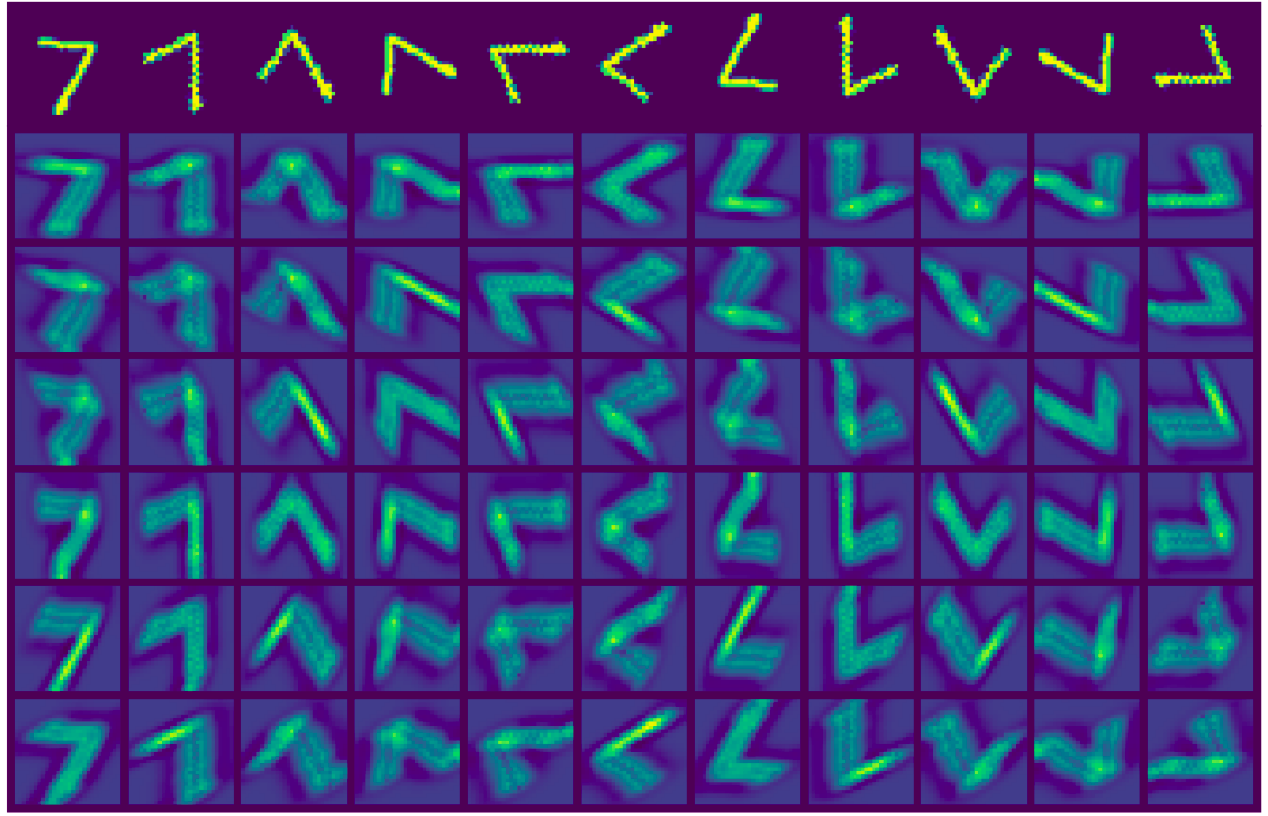
\includegraphics[width=0.6\textwidth]{Images/chebconv_filters.png}
    \caption{Rotation equivariance of a Kaiming initialized $SE(2)$ Chebyshev convolutional layer. Rotate an input image then convolve it is equivalent to convolve the original image then rotate and roll it.}
    \label{fig:7_filters}
\end{figure*}

\paragraph{Spatial pooling and unpooling layers.} Graph pooling is a central component of a myriad of graph neural network architectures. Producing coarsened graphs from a finer graph have two main advantages: first, it reduces the computational cost, and second, it could improve performance by reducing the overfitting effect and adding a multiscale perspective. As an inheritance from traditional CNNs, most approaches formulate graph pooling as a cluster assignment problem, extending local patches' idea in regular grids to graphs \citep{dhillon2007weighted, ying2018hierarchical, khasahmadi2020memory, mesquita2020rethinking}. We propose similar operations based on the spatial domain and involving two steps. First, each sample is assigned to a cluster that will correspond to the output sample; this is the down- (resp. up-) sampling phase.\footnote{Altough down- and up-samplings are naturally defined on the Euclidean grid, this task is more complicated on the sphere. However, using an icosahedron decomposition of the sphere, we make it more natural as down- and up-sampling consists of decreasing or increasing the subdivision level.}  Then, each cluster is reduced (resp. expanded) according to a given scheme (e.g. maximum, average or random); this is the reduction (resp. expansion) phase. With well-designed down- and up-sampling schemes, we can make this type of layer equivariant to any group transformation as the reduction and expansion phase are permutation-invariant operations.


\begin{figure*}[h!] 
    \centering
    \begin{subfigure}[b]{0.48\textwidth}
        \centering
        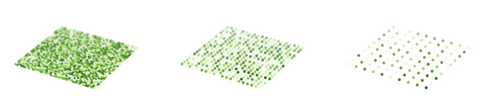
\includegraphics[width=\textwidth]{Images/r2_pooling.png}
        \caption{R2RandPool}
    \end{subfigure}
    \hfill
    \begin{subfigure}[b]{0.48\textwidth}
        \centering
        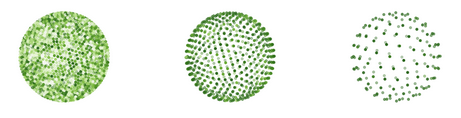
\includegraphics[width=\textwidth]{Images/s2_pooling.png}
        \caption{S2MaxPool}
    \end{subfigure}
    \hfill
    \begin{subfigure}[b]{0.48\textwidth}
        \centering
        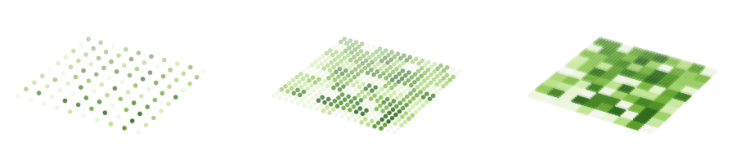
\includegraphics[width=\textwidth]{Images/r2_unpooling.png}
        \caption{R2RandUnpool}
    \end{subfigure}
    \hfill
    \begin{subfigure}[b]{0.48\textwidth}
        \centering
        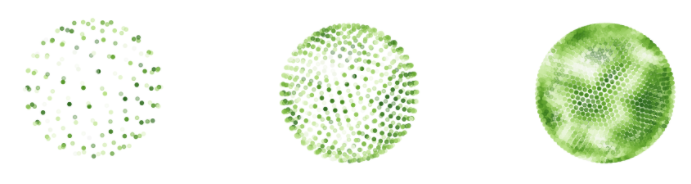
\includegraphics[width=\textwidth]{Images/s2_unpooling.png}
        \caption{S2AvgUnpool}
    \end{subfigure}
    \caption{Spatial pooling and unpooling layers.}
    \label{fig:pooling}
\end{figure*}

\paragraph{Global pooling and point-wise operations.} When the neural network does not need to be equivariant but invariant (e.g. classification task), it is common to rely on a global pooling layer (or simply projection layer). This layer reduces the d-dimensional signal on the graph's vertices to a d-dimensional vector of features synthesising the information on the whole graph. As a permutation-invariant operation, such a layer does not break the equivariance property of the neural network, but it leads to a loss of information in terms of the group transformation. Finally, point-wise operations do not affect the equivariance of a neural network. Hence, we can use as many activation functions as we need without affecting the equivariance property.


\section{Experiments} \label{sec:experiments}

In this experiments' section, we aim at showing the benefits of using tunable anisotropic kernels, which is the main contribution of our work. We are conscient that some improvements could be made optimizing the hyper-parameters of the models \citep{yu2020hyper}, using high-capacity networks or via a more advanced training process with a learning weight scheduler, but this is not the goal of our work. To illustrate the adaptability of our approach to different tasks, we evaluate our models on image classification and image segmentation tasks. In the first bunch of experiments, we try to motive anisotropic kernels on the whole Lie group. By varying the anisotropies, we show the existence of a sweet spot, both for the spatial anisotropy parameter $\varepsilon$ and the orientation anisotropy parameter $\xi$. In the second bunch of experiments, we show that even if we add a new orientation dimension, our method remains scalable using a proper implementation.

Our implementation is fully PyTorch \citep{pytorch} and available at \url{https://github.com/ebekkers/GroupEquivariantChebNets}. We perform all the experiments on a single GeForce GTX 1080 Ti GPU and track them with Weights \& Biases \citep{wandb}. The details of the experiments are presented in the appendix \ref{app:experiment_details}.

\subsection{Why using tunable anisotropic kernels?} 

As introduced in section \ref{sec:anisotropic_manifold_graph}, the anisotropic kernels are tunable via the parameters $\varepsilon$ and $\xi$\footnote{As the $\xi$ parameter should depend on the spatial and orientation resolutions, we use the following parameterisation:
\begin{equation}
\xi = 170\alpha \frac{|\mathcal{V}_o|}{|\mathcal{V}_s|}
\end{equation}
Setting $\alpha = 2$ yields to a 40/60 distribution of neighbors on the spatial and orientation domains.}
of the Riemannian metric, respectively responsible for the spatial and orientation anisotropies. We ran different experiments with a Wide Residual architecture \citep{zagoruyko2016wide} on CIFAR10 \citep{krizhevsky2009learning}, varying the spatial and orientation anisotropic parameters. 

\begin{figure*}[h!] 
    \centering
    \begin{subfigure}[b]{0.48\textwidth}
        \centering
        \caption{Test-accuracy against orientation anisotropies}
        \label{fig:sweet_spot_orientation}
        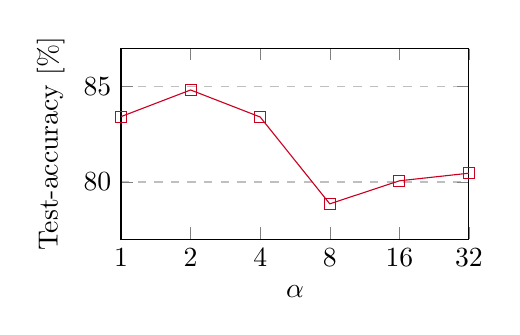
\begin{tikzpicture}
        \begin{axis}[
            xlabel={$\alpha$},
            xmode=log,
            log ticks with fixed point,
            ylabel={Test-accuracy [\%]},
            xmin=1, xmax=32,
            ymin=77, ymax=87,
            xtick={1,2,4,8,16,32},
            ytick={80, 85},
            legend pos=north east,
            ymajorgrids=true,
            grid style=dashed,
            height=4cm,
            width=6cm
        ]
        \addplot[
            color=color1,
            mark=square,
            ]
            coordinates {
            (1,83.43)(2,84.83)(4,83.41)(8,78.85)(16,80.06)(32,80.46)
            };
        \end{axis}
        \end{tikzpicture}
    \end{subfigure}
    \hfill
    \begin{subfigure}[b]{0.48\textwidth}
        \centering
        \caption{Test-accuracy against spatial anisotropies}
        \label{fig:sweet_spot_spatial}
        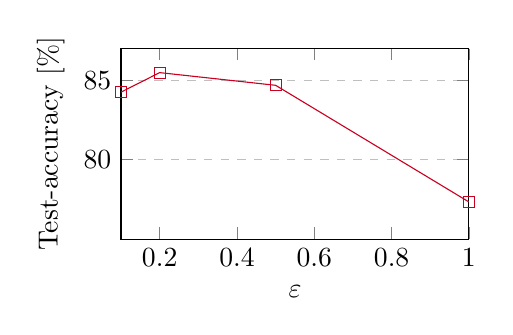
\begin{tikzpicture}
        \begin{axis}[
            xlabel={$\varepsilon$},
            ylabel={Test-accuracy [\%]},
            xmin=0.1, xmax=1.0,
            ymin=75, ymax=87,
            xtick={0,0.2,0.4,0.6,0.8,1.0},
            ytick={80, 85},
            legend pos=north east,
            ymajorgrids=true,
            grid style=dashed,
            height=4cm,
            width=6cm
        ]
        \addplot[
            color=color1,
            mark=square,
            ]
            coordinates {
            (0.1,84.26)(0.2,85.49)(0.5,84.69)(1.0,77.34)
            };
        \end{axis}
        \end{tikzpicture}
    \end{subfigure}
    \caption{Empirical proof of existence of sweet spots for data-dependent anisotropic parameters.}
\end{figure*}

\paragraph{Orientation anisotropy.} The orientation anisotropy $\xi$ controls how intensively orientation layers are connected. At the limit $\xi \to \infty$, orientation layers are decoupled. It is like test-time augmentation with rotations: running a CNN working with one anisotropic Laplacian (e.g., only vertically aligned filters) and testing the network for different input rotations before averaging the output. The other extreme $\xi \to 0$ keeps all layers equally close to each other, and features are essentially identified with just a spatial coordinate. A disadvantage of this method is that it requires many neighbours to get an excellent spatial resolution since the neighbourhood is necessarily distributed on all orientation layers (typically, we should use $\tilde{K} = |\mathcal{V}_o| K$ neighbours). For reasonable values of $\xi$, interactions between orientation layers take place. Figure \ref{fig:sweet_spot_orientation} is evidence of the existence of a sweet spot for this parameter in the range of reasonable values. At the moment, we expect with no certainty that this parameter could be set \emph{a priori} of the data, only considering the data resolution. From now on, as a rule of thumb, we set $\xi$ such that we roughly reach the 40/60 neighbourhood ratio. Each vertex has approximately 40\% of its neighbours on the same orientation layer and 60\% on different ones.

\paragraph{Spatial anisotropy.} The spatial anisotropy $\varepsilon$ regulates the anisotropy of the kernels on the spatial domain. For $\varepsilon = 1$, the Riemannian metric is spatially isotropic; all directions are treated equally. At the limit $\varepsilon \to 0$, the main direction has a minimal cost, and the resulting filters are highly spatially anisotropic. In figure \ref{fig:sweet_spot_orientation} we observe that using anisotropic filters instead of isotropic ones is relevant, as we almost get an 8\% test-accuracy improvement. Unlikely the orientation anisotropic parameter, in our opinion, this parameter is highly data-dependent. Between two different datasets, the required spatial anisotropic can change drastically.\footnote{Just think of a dataset with cats  and dogs' images and the same dataset with the same but elongated images, in one direction. The orientation anisotropy would remain identical for both but the spatial one would be adapted.}



\subsection{How scalable is the method?}

Scalability is often an important limitation of graph- and group-based neural networks. By adding an orientation dimension, we do not run from this rule as we necessarily increase the number of vertices of the anisotropic manifold graphs. Nevertheless, with some smart tips, we push the limits and evaluate our models on an image classification task on STL10 \citep{coates2011analysis} and an image segmentation task on ClimateNet \citep{kashinath2021climatenet}.\footnote{The original STL10 and ClimateNet images respectively lie in $\mathbb{R}^{9216 \times 3}$ and $\mathbb{R}^{10242 \times 16}$.} We show the great adaptability of our method by using a Wide Residual architecture \citep{zagoruyko2016wide} on STL10 and a U-Net-like network \citep{ronneberger2015u} on ClimateNet.

\begin{table}[h!]
\centering 
\caption{Mean of test performance and training duration on ClimateNet and STL10. Errorbars are 1 standard deviation computed over 5 trials.}
\begin{tabular}{c c c c c}
\toprule
 & \multicolumn{2}{c}{ClimateNet} & \multicolumn{2}{c}{STL10} \\
$\varepsilon$ & Test F1 & Duration & Test accuracy & Duration \\
\midrule
$1$ & $\boldsymbol{85.62 \pm 0.09 \%}$ & $\sim \SI{2}{\day}$ & $68.98 \pm 0.56 \%$ & $\sim \SI{9}{\hour}$ \\
$0.1$ & $85.25 \pm 0.19 \%$ & $\sim \SI{7}{\day}$ & $\boldsymbol{74.02 \pm 1.10 \%}$ & $\sim \SI{16}{\hour}$ \\
\bottomrule
\end{tabular}
\end{table}

This experiment illustrates the main limitation of our approach: its poor scalability. Our anisotropic models are costly in terms of time and memory because of the sizes of graphs and features maps. Operations are time consuming and memory demanding. Using an intelligent implementation is not an option but a requirement. However, the good news is that once the scalability wall has been passed through, our method has excellent capabilities and clearly illustrates the benefits of using anisotropic tunable kernels. Indeed, while on ClimateNet the use of anisotropic kernels is neither beneficial nor detrimental, the difference in performance on STL10 is significant.

\section{Conclusion} \label{sec:conclusion}

We conclude this work with a few comments on the potential impact of our approach in the trendy field of geometric deep learning.

\paragraph{Scope.} As it is able to model any Lie group, our method is extendable to many datasets. Using $SE(2)$ group, we can get a roto-translation equivariant neural network for $2D$ images or videos. With the higher dimensional group $SE(3)$, the method can solve a task involving 3-dimensional shapes requiring roto-translation equivariance. On the sphere and using the group $SO(3)$, the method can deal with meteorological or cosmological data while preserving rotation equivariance. For each task, it is necessary to exist an orientation axis, based on which we can steer the anisotropic kernels.

\paragraph{Limitations.} The main weakness of our method is its high memory requirements. By adding an orientation axis, we significantly enlarge the feature maps. As a result, anisotropic graph manifolds are memory-heavier than isotropic ones and prone to overfitting and slowdown during forward and backward pass. Nevertheless, with the emergence of graph-based machine learning algorithms, we expect cutting-edge technologies to become more performant on graph data. We hope the advances in quantum machine learning will help alleviate this problem in the next few years. At the present moment, it is still possible to use some dedicated libraries such as PyKeops \citep{charlier2020kernel}. This memory-efficient library relies on the concept of symbolic matrices and takes advantage of CUDA registers' structure to bypass costly memory transfers and achieve optimal runtimes on a wide range of applications. Another difficulty of our method is its high number of hyper-parameters on which we only have some rule of thumb to set them. The graph connectivity requires a tradeoff between efficiency and quality of the group approximation. The anisotropic parameters require a deep analysis of the dataset and some intuition about the necessity of using anisotropic kernels and how strong we should set these anisotropies. The similarity kernel bandwidth is also hard to set. With a systematic hyper-parameter optimization \citep{yu2020hyper}, we can find an optimal combination, but it requires many computational resources.

\paragraph{Future research.} As it has been mentioned earlier, it could be interesting to launch a deep ablation study about the model's hyper-parameters (orientation resolution, anisotropies, graph connectivity, etc.). In particular, some questions remain. Do we need to use an higher graph connectivity for an anisotropic GEChebNet than for an isotropic one, as the neighborhood of a vertex is spread over several orientation layers? How to easily set intensities of the spatial anisotropies, could we use an heuristic for that? How strong should be the connection between orientation layers? Extend the approach to higher dimensional Lie groups and arbitrary shapes and surfaces with and orientation space.

\haguettaz{convergence of graph laplacian to anisotropic Laplace Beltrami operator?}


\begin{ack}
This paper is a collaborative effort between the LTS2 (EPFL) and the AMLab (UvA). Hence, we wish to express our deepest gratitude to both schools for this amazing opportunity. We also thank all the people working at SURFsara\footnote{\url{https://userinfo.surfsara.nl/}}, for letting us use Lisa, their excellent computation service. 
\end{ack}

\clearpage
\bibliographystyle{plainnat}
\bibliography{bibliography}

%%%%%%%%%%%%%%%%%%%%%%%%%%%%%%%%%%%%%%%%%%%%%%%%%%%%%%%%%%%%
\clearpage
\section*{Checklist}

%%% BEGIN INSTRUCTIONS %%%
The checklist follows the references.  Please
read the checklist guidelines carefully for information on how to answer these
questions.  For each question, change the default \answerTODO{} to \answerYes{},
\answerNo{}, or \answerNA{}.  You are strongly encouraged to include a {\bf
justification to your answer}, either by referencing the appropriate section of
your paper or providing a brief inline description.  For example:
\begin{itemize}
  \item Did you include the license to the code and datasets? \answerYes{See Section xxx.}
  \item Did you include the license to the code and datasets? \answerNo{The code and the data are proprietary.}
  \item Did you include the license to the code and datasets? \answerNA{}
\end{itemize}
Please do not modify the questions and only use the provided macros for your
answers.  Note that the Checklist section does not count towards the page
limit.  In your paper, please delete this instructions block and only keep the
Checklist section heading above along with the questions/answers below.
%%% END INSTRUCTIONS %%%

\begin{enumerate}

\item For all authors...
\begin{enumerate}
  \item Do the main claims made in the abstract and introduction accurately reflect the paper's contributions and scope?
    \answerYes{See Section~\ref{sec:introduction}}
  \item Did you describe the limitations of your work?
    \answerYes{See Section~\ref{sec:conclusion}}
  \item Did you discuss any potential negative societal impacts of your work?
    \answerTODO{}
  \item Have you read the ethics review guidelines and ensured that your paper conforms to them?
    \answerTODO{}
\end{enumerate}

\item If you are including theoretical results...
\begin{enumerate}
  \item Did you state the full set of assumptions of all theoretical results?
    \answerYes{See Section~\ref{sec:method}}
	\item Did you include complete proofs of all theoretical results?
    \answerYes{We refer the reader to original publication with proofs.}
\end{enumerate}

\item If you ran experiments...
\begin{enumerate}
  \item Did you include the code, data, and instructions needed to reproduce the main experimental results (either in the supplemental material or as a URL)?
    \answerYes{See Section~\ref{sec:method}}
  \item Did you specify all the training details (e.g., data splits, hyperparameters, how they were chosen)?
    \answerYes{See Section~\ref{sec:experiments}}
	\item Did you report error bars (e.g., with respect to the random seed after running experiments multiple times)?
    \answerYes{See Section~\ref{sec:experiments}}
	\item Did you include the total amount of compute and the type of resources used (e.g., type of GPUs, internal cluster, or cloud provider)?
    \answerYes{See Section~\ref{sec:experiments}}
\end{enumerate}

\item If you are using existing assets (e.g., code, data, models) or curating/releasing new assets...
\begin{enumerate}
  \item If your work uses existing assets, did you cite the creators?
    \answerYes{See Section~\ref{sec:experiments}}
  \item Did you mention the license of the assets?
    \answerNA{}
  \item Did you include any new assets either in the supplemental material or as a URL?
    \answerNA{}
  \item Did you discuss whether and how consent was obtained from people whose data you're using/curating?
    \answerNA{}
  \item Did you discuss whether the data you are using/curating contains personally identifiable information or offensive content?
    \answerNA{}
\end{enumerate}

\item If you used crowdsourcing or conducted research with human subjects...
\begin{enumerate}
  \item Did you include the full text of instructions given to participants and screenshots, if applicable?
    \answerNA{}
  \item Did you describe any potential participant risks, with links to Institutional Review Board (IRB) approvals, if applicable?
    \answerNA{}
  \item Did you include the estimated hourly wage paid to participants and the total amount spent on participant compensation?
    \answerNA{}
\end{enumerate}

\end{enumerate}

%%%%%%%%%%%%%%%%%%%%%%%%%%%%%%%%%%%%%%%%%%%%%%%%%%%%%%%%%%%%

\appendix

\section{Background} \label{app:background}

\subsection{Riemannian geometry} \label{app:riemannian_geometry}

Riemannian geometry is a part of differential geometry that studies Riemannian manifolds, smooth manifolds equipped with a Riemannian metric. A manifold $\mathcal{M}$ is a generalization and abstraction of the notion of a curved surface. It is a topological set that is modeled closely on Euclidean space locally but may vary widely in global properties. It means for each $p \in \mathcal{M}$, we can associate a tangent space $T_p(\mathcal{M}) \subseteq \mathbb{R}^d$, corresponding to the union of all tangent vectors of differentiable curves passing through $p$. Consequently, at any point $p \in \mathcal{M}$, the tangent space $T_p(\mathcal{M})$ is spanned by a basis $\{\partial_{x_i, p} \}_{i=1}^N$:
\begin{equation}
T_p(\mathcal{M}) = \{ \dot{\gamma}(0) | \gamma : \mathbb{R} \to \mathcal{M} \in \mathcal{C}^1 \text{and } \gamma(0) = p\} = \spn\{\partial_{x_i,p} \}_{i=1}^N.
\end{equation}
A Riemannian manifold is a differentiable manifold $\mathcal{M}$ with a Riemannian metric $\mathcal{R}$, a 2-tensor field, such that at each $p \in \mathcal{M}$, we have a function $\mathcal{R}|_p : T_p (\mathcal{M}) \times T_p(\mathcal{M}) \to \mathbb{R}$ which is symmetric and positive definite. At each $g \in G$, the Riemannian metric can be expressed by its local representation, a symmetric positive definite matrix $\boldsymbol{R}_p$ whose components are given by:
\begin{equation}
r_{ij}(p) = \mathcal{R}|_p (\partial_{x_i, p}, \partial_{x_j, p}).
\end{equation}
In the following we consider Riemannian metric with  diagonal local representation at the origin $e$, that is:
\begin{equation}
r_{ij}(e) = \left\{
    \begin{array}{ll}
        r_{i} & \text{if } i = j  \\
        0 & \text{otherwise}
    \end{array}
\right..
\end{equation}
The Riemannian metric induces an inner product, such that for any $u = u^i \partial_{x_i, e}$ and $v = v^i \partial_{x_i, e}$, we have $\langle u, v \rangle_{\mathcal{R}(e)} = u^i r_i v^i$ and $|| u ||_{\mathcal{R}(e)}^2 = u^i r_i u^i$. Between each pair of points $p$ and $q$ of a Riemannian manifold, we define their Riemannian distance as the length of the shortest curve connecting the two points (a.k.a. geodesic). More formally, we have:
\begin{equation}
d(p, q) = \inf_{\gamma \in \mathcal{C}^\infty_{p, q}} \int_0^1 ||\dot{\gamma}(\tau)||_{\mathcal{R}_{\gamma(\tau)}} d\tau,
\end{equation}
where $\mathcal{C}^\infty_{p, q} = \{ \gamma : [0, 1] \to \mathcal{M} | \gamma \in \mathcal{C}^\infty, \gamma(0) = p,  \gamma(1) = q\}$. An more convenient way to define the Riemannian between two points is via the exponential and logarithmic Riemannian maps (Figure \ref{fig:explogmap}). The Riemannian exponential map $\exp_p T_p(\mathcal{M}) \to \mathcal{M}$ is defined as:
\begin{equation}
\exp_p (v) = \gamma_{p, v}(1) ,\qquad (\text{and by extension } \exp_p (tv) = \gamma_{p, v}(t)),
\end{equation}
where $\gamma_{p,v}(1)$ is the unique Riemannian geodesic starting at $p \in \mathcal{M}$ with initial velocity $v \in T_p(\mathcal{M})$. We can interpret the exponential map as follows. Let’s choose any direction in our tangent space and follow it with a step forward. We make sure to take the shortest path and end up at a new point. This process is what we called the exponential map.\footnote{It comes from the fact that all these tiny steps magically resemble the series expansion of the exponential function.} The inverse mapping of the exponential map, the logarithmic map $\log_p : \mathcal{M} \to T_p(\mathcal{M})$ will map an element $p \in \mathcal{M}$ to the smallest vector $v = \log_p q \in T_p(\mathcal{M})$ as measured by the Riemannian metric such that $q = \exp_p v \in \mathcal{M}$. 

\begin{figure*}[h!]
    \centering
    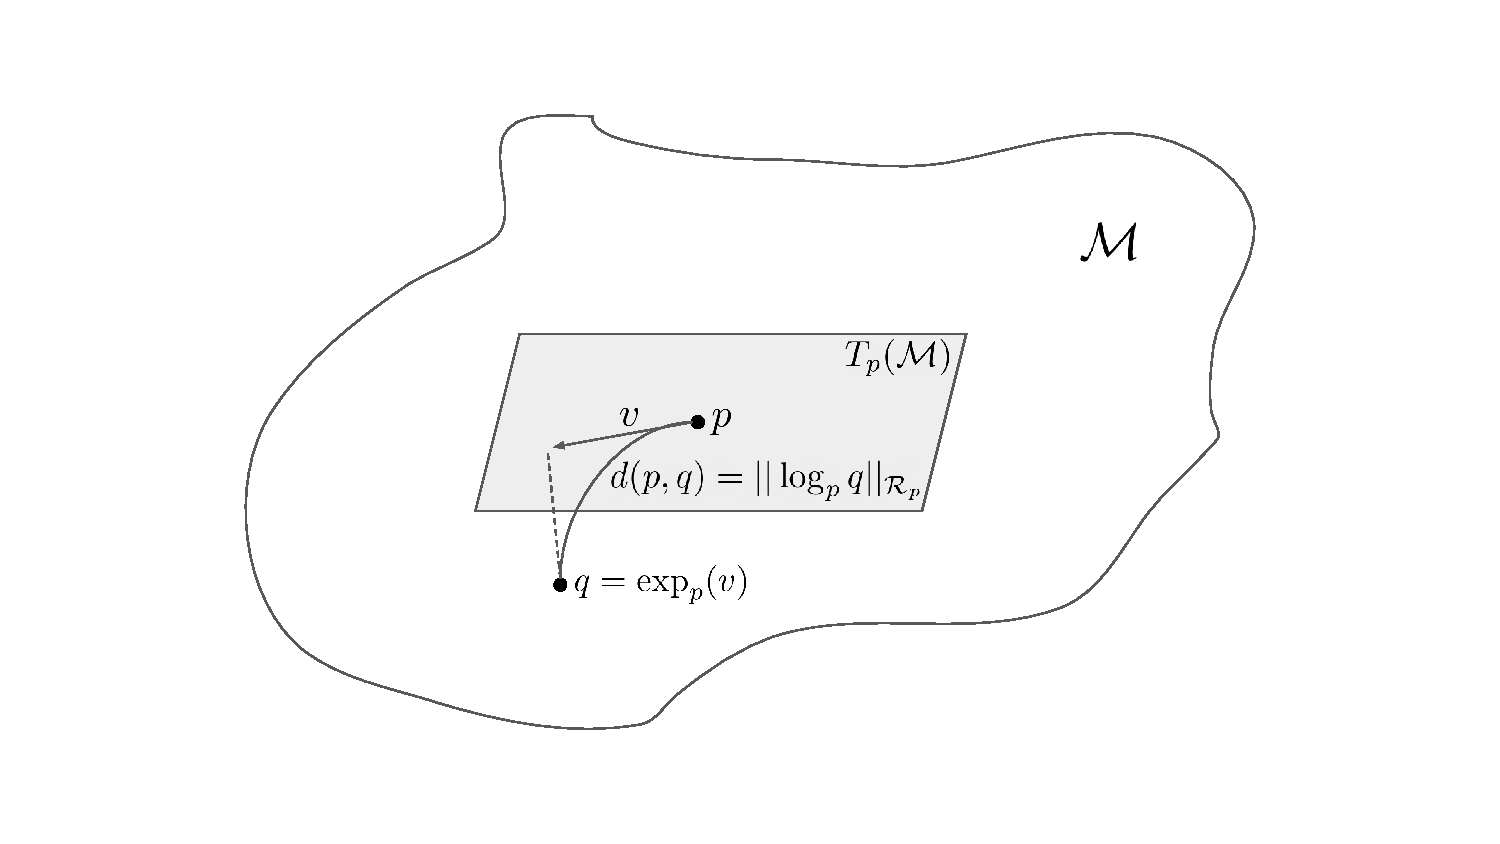
\includegraphics[width=\textwidth]{Images/distexplog.pdf}
    \caption{Riemannian exponential map $\exp_p : T_p(\mathcal{M}) \to \mathcal{M}$ and Riemannian logarithmic map $\log_p : \mathcal{M} \to T_p(\mathcal{M})$.}
    \label{fig:explogmap}
\end{figure*}


\subsection{Group theory} \label{app:group_theory}

A rigorous investigation of an operator property of equivariance under a group transformation, require a bit of knowledge in group theory. A group $(G, \cdot)$ is a set $G$ equipped with a binary operation $\cdot : G \to G$ called group product, satisfying the four group axioms (closure, associativity, identity element and inverse elements). To map the structure of the group to some mathematical object, one requires a representation. We define $H$ as the vector space to which our mathematical object belongs and $\mathcal{B}(H)$ the space of bounded linear invertible operators $H \to H$. A representation $\mathcal{V} : G \to \mathcal{B}(H)$ maps a group element to an operator such that the identity element, the group product and the group inverse are preserved. We define the left-regular representation $\mathcal{L}_g$ on the (infinite-dimensional) vector space of functions $G \to \mathbb{R}^d$ via:
\begin{equation}
(\mathcal{L}_g \circ f )(h) = f(g^{-1}h),
\end{equation}
with $f : G \to \mathbb{R}^d$ a function on the group $G$ and $g, h$ elements of the group $G$. Using this group representation, we can formally define the left-invariance (a.k.a. equivariance).

\begin{definition}[Equivariance] \label{def:equivariance}
An operator $\Phi : \mathcal{X} \to \mathcal{Y}$ from one vector space to the other is equivariant (or left-invariant under group transformation) if it satisfies the following property:
\begin{equation}
\mathcal{L}'_g \circ \Phi = \Phi \circ \mathcal{L}_g, \qquad \forall g \in G.
\end{equation}
\end{definition}

Equivariance can be realized in many ways, and in particular, the group representations $\mathcal{L}_g$ and $\mathcal{L}'_g$ need not be the same, as they act on different spaces $\mathcal{X}$ and $\mathcal{Y}$. Note that the familiar concept of invariance is a special kind of equivariance where  $\mathcal{L}_g'$ is the identity transformation for all element $g$ of the group $G$. 

% We define the equivariance error, a measure of the equivariance of an operator.

% \begin{definition}[Equivariance error] \label{def:equiv_err}
% Let $\Phi : \mathbb{L}_2(G) \to \mathbb{L}_2(G)$ be an operator and $g$ an element of a group $G$ with left regular representation $\mathcal{L}_g$. The equivariance error of the operator $\Phi$ is given by:
% \begin{equation}
% \varepsilon(g, f) = \frac{|| (\mathcal{L}'_g \circ \Phi )(f) - ( \Phi \circ \mathcal{L}_g) (f)||_2^2}{|| (\mathcal{L}'_g \circ \Phi )(f)||_2^2}, \qquad f \in \mathbb{L}_2(G).
% \end{equation}
% \end{definition}

A Lie group is a continuous group whose group elements are parameterized by a finite-dimensional differentiable manifold. In essence, this means that a Lie group is a group to which we can apply differential geometry. From now on, we also assume the group manifold is equipped with a Riemannian metric, that is it is Riemannian manifold. To each element $g$ of $G$, we can associate a tangent space $T_g(G)$, which is spanned by a basis of left-invariant vectors denoted by $\{\mathcal{A}_i|_g\}_{i=1}^n$. We write $T_g(G) = \spn\{\mathcal{A}_1|_g, \dots, \mathcal{A}_n|_g\}$ and we can express tangent vectors $\dot{\gamma}(t)$ of $T_g(G)$ in this basis via $\dot{\gamma}(t) = c^i(t) \mathcal{A}_i|_{\gamma(t)}$.

Moreover, because this frame of basis vector is left-invariant, the coefficients $c_i(t)$ remain unchanged if the curve is moved by applying left group product. The tangent space at the origin $T_e(G)$ is spanned by a basis $\{A_i\}_{i=1}^n$ where $A_i = \mathcal{A}_i|_e$. We make a subtle difference in notation between $\mathcal{A}$ and $A$, where $\mathcal{A}$ represents a whole vector field and $\mathcal{A}|_g$ represents the vector at location $g$. The straight $A$ is used to indicate a vector in the Lie algebra, the tangent space at the origin. Via the push-forward $(L_g)_*$, we can generate a whole vector space by picking a vector in the Lie algebra and transporting tangent vectors from $\dot{\gamma}(0) \in T_e(G)$ to $g \cdot \dot{\gamma}(0) \in T_g(G)$ using:
\begin{equation}
\mathcal{A}_i|_g = (L_g)_* A_i , \qquad \forall g \in G.
\end{equation}

The left-invariant frame of basis vectors could also be interpreted as the directional derivative of functions defined on the group $G$. At any element $g$, the value of the directional derivative of a function $f$ defined on $G$ can be computed using the push-forward operation:
\begin{equation}
\mathcal{A}_i|_g f = (L_g)_* \mathcal{A}_i|_e f := \mathcal{A}_i|_e (f \circ L_{g^{-1}}),
\end{equation}
so $\mathcal{A}_i|g f$ represents the directional derivative along the vector field at location $g$, which can be defined by translating the function back to the origin via $L_{g^{-1}}$ and compute the derivative at the origin along the direction specified by $\mathcal{A}_i|_e$. In the above $L_g h:= g h$.
 
The Laplace-Beltrami operator, the generalization to Riemannian manifold of the Laplace operator\footnote{Another equivalent definition in local coordinates exists too. It explicitly takes into account the Riemannian metric tensor field $\mathcal{R}$ previously defined. Here we use a more compact definition but using the subscript $\mathcal{R}(g)$ to indicate that the Laplace-Beltrami operator depends on the location on the Riemannian manifold and the Riemannian metric tensor field.} is defined below. 
\begin{definition}[Laplace-Beltrami operator] \label{def:laplace_beltrami}
Let $g$ be an element of the Lie group $(\mathcal{M}, \cdot)$. The Laplace-Beltrami operator on the Riemannian manifold $\mathcal{M}$ is defined as 
\begin{equation}
\Delta_{\mathcal{R}(g)} = \dive (\nabla_{\mathcal{R}(g)})
\end{equation}
\end{definition}

Using the left-invariant frame of basis vectors as directional differential operators, we can define the gradient, expressed as a vector relative to the basis $\mathcal{A}_i|_g$, of a function $f : G \to G$:
\begin{equation}
\nabla_{\mathcal{R}(g)} f = \mathbf{R}_{g}^{-1} (\mathcal{A}_1|_g f, \dots, \mathcal{A}_n|_g f)^\top,
\end{equation}
where $\mathbf{R}_{g}$ is the Riemannian metric tensor defined relative to the basis $\mathcal{A}_i$, that corrects for local scaling and shrinking of the manifold as measured by the metric tensor.
The divergence of a vector field $F : G \to \mathbb{R}^n$ is the operator:
\begin{equation}
\dive(F) = \sum_{i=1}^n \mathcal{A}_i|_g F_i.
\end{equation}

The Laplace-Beltrami operator depends on a Riemannian metric tensor, which describes how lengths of vectors should be measured in different directions, and in the Laplace-Beltrami operator, it rescales the derivates accordingly. While the usual Laplacian is isotropic (derivatives are threated the same in each direction), the Laplace-Beltrami operator can be anisotropic due to the Riemannian metric that is used.

\begin{theorem}[Left-invariance of the Laplace-Beltrami operator] \label{thm:equiv_laplace_beltrami}
The Laplace-Beltrami operator $\Delta_{\mathcal{R}(g)}$ is left-invariant and satisfies:
\begin{equation}
\Delta_{\mathcal{R}(g)} = (L_g)_* \Delta_{\mathcal{R}(e)}.
\end{equation}
\end{theorem}


A Lie algebra $\mathfrak{g}$ is a vector space (here the tangent space at the identity element $T_e(G)$) that is endowed with a binary operator called the Lie bracket or commutator $[\cdot, \cdot] : T_e(G) \times T_e(G) \to T_e(G)$ that is bilinear, alternative and satisfies the Jacobi identity. Conceptually, the Lie bracket $[A, B]$ of two vector fields $A, B$ is the derivative of $B$ along the flow generated by $A$.\footnote{Two vector fields are commutative (zero Lie bracket) if and only if its flows are too, in the sense that there is no difference starting at one point $p$, traveling a time $t_a$ over the flow of $A$ and then a time $t_b$ over the flow of $B$, or, instead, traveling first $t_b$ over the flow of $B$ and then $t_a$ over the flow of $A$.} In the following, we take $\{A_i\}_{i=1}^n$ with $A_i = \mathcal{A}_i|_e$ as Lie Algebra and get left-invariant vector fields via the push-forward operation. 

The Lie group exponential and logarithmic maps define the mappings between the group and the tangent space. The exponential map on a Lie group can be thought of as picking a vector $A$ in the Lie algebra, construct a left-invariant vector field $\mathcal{A}$ via the push-forward operator, and follow this vector field by taking infinitesimal steps along the direction indicated by the vector field. Integrating along the vector field defined by $A$ for unit time brings to some point $g \in G$. So $g = \exp A$, where $\exp: \mathfrak{g} \to G$.\footnote{Note that Riemannian and Lie group exponential maps are different. For the general Riemannian exponential map, the vector field along which we compute the path integral is defined by the Riemannian metric. In the Lie group exponential map, the vector field is defined by the push forward of left-multiplication. The curves defined by the path integrals in the Riemannian exponential are known to be geodesics. The exponential curves in the Lie group case are "straight curves" with respect to a moving frame of reference but are not necessarily geodesics. The Riemannian and Lie group exponential maps only coincide when the Riemannian metric is both left and right invariant (see Section 4.5 in \citet{bekkers2017thesis}).}



\subsection{Graph theory} \label{app:graph_theory}

Graphs are generic data representation forms that are useful for describing the geometric structure of data domains \citep{west1996introduction}. More formally, we define a graph $\mathcal{G}$ as a structure modeling a finite set of interactions called edges $\mathcal{E}$ between a finite set of objects called vertices $\mathcal{V}$. In the following, we denote by $|\mathcal{V}|$ the number of vertices and by $|\mathcal{E}|$ the number of edges. We denote $v_i$ the $i$-th vertex and $e(v_i, v_j)$ the potential edge from $v_i$ to $v_j$. We call the neighborhood of the vertex $v_i$ the set of vertices connected to $v_i$ by an edge and denote it by $\mathcal{N}(v_i)$. More generally, we write $\mathcal{N}^k(v_i)$ for the $k$-hops neighborhood of vertex $v_i$, that is, the set of vertices connected to $v_i$ with a path of at most $k$ edges. In some cases, it can be useful to add weights on graph edges. In general, the weights can take any value. Nevertheless, in this thesis, we assume weights in the range $[0, 1)$ and measuring the similarity rather than the distance. When the edges' weights are not naturally defined by an application, a common way to define them is to apply a kernel $\mathfrak{K} : \mathbb{R}_+ \to [0, 1)$ on the distance between connected nodes. For theoretical convergence results, we use a Gaussian weighting scheme: 
\begin{equation}
w(v_i, v_j) =
\left\{ 
\begin{array}{ll}
\exp \left(- \frac{d^2(v_i, v_j)}{4t}\right) & \text{if } e(v_i, v_j) \in \mathcal{E} \\
0 & \text{otherwise}
\end{array}
\right.,
\end{equation}
where $d(v_i, v_j)$ denotes the (Riemannian) distance between vertices $v_i$ and $v_j$ and $t$ is a positive real number called bandwidth of the Gaussian kernel. From now on, we furthermore assume that the graphs are undirected and without self-loop.

The field of signal processing on graphs merges algebraic and spectral graph theoretic concepts with computational harmonic analysis to process such signals on graphs \citep{shuman2013gsp}. A signal on a graph is a function $f : \mathcal{V} \to \mathbb{R}^d$, mapping each vertex of the graph to a $d$-dimensional real valued vector. In matrix form, this signal is a $|\mathcal{V}| \times d$ real valued matrix $\boldsymbol{f}$ whose rows are given by $\boldsymbol{f}_i = f(v_i) \in \mathbb{R}^d$. 

An essential object in graph signal processing is the Laplacian operator. Under some specific conditions that we will state later, it can be interpreted as a discrete version of the Laplace-Beltrami operator.
\begin{definition}[Symmetric normalized Laplacian] \label{def:graph_laplacian}
Let $\mathcal{G}$ be an undirected weighted graph without self-loops. The symmetric normalized Laplacian $\boldsymbol{\Delta}$ is the $|\mathcal{V}| \times |\mathcal{V}|$ real valued matrix whose components are given by:
\begin{equation}
\Delta_{i, j} =
\left\{
\begin{array}{ll}
1 & \text{if } i = j \text{ and } \deg(v_i) > 0 \\
- \frac{w(v_i, v_j)}{\sqrt{\deg (v_i) \deg (v_j)}} & \text{if } i \neq j \text{ and } \deg(v_i) > 0 \\ 
0 & \text{otherwise}
\end{array}
\right..
\end{equation}
\end{definition}

Assuming a function $f$ defined on the graph vertices $\mathcal{V}$, by inspection on the components of $\boldsymbol{\Delta}^k \boldsymbol{f}$, we remark that the Laplacian acts as a $k$-op neighborhood operator. We can prove that $\boldsymbol{\Delta}$ is a symmetric positive definite matrix. Hence it admits a unique eigendecomposition of the form $\boldsymbol{\Delta} = \boldsymbol{\Phi \Lambda \Phi}^\top$ where the $j$-th column of $\Phi$ correponds to the eigenvector $\phi_j$ associated with real positive eigenvalue $\lambda_j$. In these settings, the eigenvalues are in the range $[0, 2]$ \citep{chung1997spectral}. By analogy with the Euclidean case where the Laplacian's eigenfunctions correspond to the Fourier basis, we can construct a graph Fourier basis from the eigendecomposition of the graph Laplacian, and define the graph Fourier transform and its inverse.\footnote{The existence of an inverse transform is a direct consequence of the orthonormality of the eigenvectors.}
\begin{definition}[Graph Fourier transform]
Let $\mathcal{G} = (\mathcal{V}, \mathcal{E})$ be a graph with Laplacian $\boldsymbol{\Delta}$ and let $f : \mathcal{V} \to \mathbb{R}$ be a signal defined on the graph's vertices. The graph Fourier transform $\hat{f}$ of $f$ is given by:
\begin{equation}
\hat{f}(\lambda_j) = \hat{f}_j = \{ \boldsymbol{\Phi}^\top \boldsymbol{f}\}_j = \sum_i \phi_{ij} f_i = \sum_{v_i} \phi(v_i, \lambda_j) f(v_i),
\end{equation}
and its inverse transform by:
\begin{equation}
f(v_i) = f_i = \{\boldsymbol{\Phi}  \boldsymbol{\hat{f}} \}_i = \sum_j \phi_{ij} \hat{f}_j = \sum_{\lambda_j} \phi(v_i, \lambda_j) \hat{f}(\lambda_j).
\end{equation}
\end{definition}

\clearpage

\section{Lie groups} \label{app:lie_groups}

At the moment, all the group's elements we are interested in are in 1-1 correspondence with elements of the 3-dimensional general linear group $GL(3)$, the group of $3 \times 3$ real matrices. We will use this representation since working with matrices is more convenient in general. Moreover the Lie group exponential and logarithm coincide with the matrix exponential and logarithm.

For the roto-translation group  $SE(2)$, the spatial part corresponds to the planar translations and the orientation part to the rotation angles. Group elements $g \in SE(2)$ are given in matrix formulation by:
\begin{equation}
g = (x, y, \theta) \leftrightarrow 
\boldsymbol{G_g} = 
\left(
\begin{array}{ccc}
\cos \theta & - \sin \theta & x \\
\sin \theta & \cos \theta & y \\
0 & 0 & 1 \\
\end{array}
\right),
\end{equation}
hence the group is 3 dimensional with two parameters $x,y$ coming from the spatial space $\mathbb{R}^2$ and one orientation parameter coming from $S^1$.

The Lie algebra $\mathfrak{se}(2)$ is the set of $3 \times 3$ matrices:
\begin{equation}
\boldsymbol{A_1} = 
\left(
\begin{array}{ccc}
0 & 0 & 1 \\
0 & 0 & 0 \\
0 & 0 & 0 \\
\end{array}
\right)
, \quad
\boldsymbol{A_2} = 
\left(
\begin{array}{ccc}
0 & 0 & 0  \\
0 & 0 & 1 \\
0 & 0 & 0 \\
\end{array}
\right)
, \text{ and} \quad
\boldsymbol{A_3} = 
\left(
\begin{array}{ccc}
0 & -1 & 0 \\
1 & 0 & 0 \\
0 & 0 & 0 \\
\end{array}
\right)
\end{equation}

Naturally, it is impossible to uniformly sample elements on this group because the $\mathbb{R}^2$ space is infinite. Adding boundaries to the euclidean space, we get the $[0, 1)^2$ space, which is not homogeneous anymore, but on which it is possible to uniformly sample $|\mathcal{V}_s|$ elements. Because we are considering anisotropic Laplace-Beltrami operators which are symmetric under reflections, it is sufficient to sample the rotation angles $\theta$ only in in the range $[-\pi/2, \pi/2)$ instead of the full circle $S^1$.

As defined by its Lie algebra, the matrix logarithm related to an element of the $SE(2)$ group has the form:

\begin{equation}
\log_e \boldsymbol{G}_g = 
\left(
\begin{array}{ccc}
0 & -c_3 & c_1 \\
c_3 & 0 & c_2 \\
0 & 0 & 0 \\
\end{array}
\right)
\end{equation}

It results that the logarithmic map $\log_e : SE(2) \to \mathfrak{se}(2)$ admits a closed form expression $\log_e g = (c_1, c_2, c_3)^\top$ with\footnote{In the isotropic case, corresponding to the $2$-d Euclidean space, one can check that using the exact same expression of the logarithmic map with $\theta = 0$ gives the Euclidean distance.}:
\begin{equation}
c_1 = \frac{\theta}{2} \left(y + x \cot \frac{\theta}{2} \right)
, \quad
c_2 = \frac{\theta}{2} \left(-x + y \cot \frac{\theta}{2} \right)
, \text{ and} \quad
c_3 = \theta.
\end{equation}


The group $SO(3)$ of all rotations about the origin of 3-dimensional Euclidean space can be split into a "spatial" part which is the sphere, and a rotation part, which is a rotation around a particular reference axis. Using $ZYZ$ representation, group elements $g \in SO(3)$ are given in matrix formulation by:
\begin{equation}
g = (\alpha, \beta, \gamma) \leftrightarrow 
\boldsymbol{G_g} = \boldsymbol{R}_{\gamma, z} \boldsymbol{R}_{\beta, y} \boldsymbol{R}_{\alpha, z},
\end{equation}
where $\alpha \in [-\pi, \pi]$, $\beta \in [-\pi/2, \pi/2]$ and $\gamma \in [-\pi, \pi]$. We view the sphere $S^2$ as the spatial part, just like we view our Earth as locally flat. $S^2$ is parametrized with Euler angles $\beta$ and $\gamma$, which are independent of $\alpha$. The rotation part is then parametrized by $\alpha$. 

The Lie algebra $\mathfrak{so}(3)$ is the set of antisymmetric $3 \times 3$ matrices:
\begin{equation}
\boldsymbol{A_1} = 
\left(
\begin{array}{ccc}
0 & 0 & 1 \\
0 & 0 & 0 \\
-1 & 0 & 0 \\
\end{array}
\right)
,\quad
\boldsymbol{A_2} = 
\left(
\begin{array}{ccc}
0 & -1 & 0  \\
1 & 0 & 0 \\
0 & 0 & 0 \\
\end{array}
\right)
, \text{ and} \quad
\boldsymbol{A_3} = 
\left(
\begin{array}{ccc}
0 & 0 & 0 \\
0 & 0 & -1 \\
0 & 1 & 0 \\
\end{array}
\right).
\end{equation}

To uniformly sample on the group $SO(3)$ is quite challenging because a perfectly uniform sampling on the sphere does not exist. Fortunately, this task has been largely studied, and many algorithms have been proposed: equiangular\footnote{Equiangular is far from uniform, but it has a sampling theorem.} \citep{driscoll1994computing}, HEALPix \citep{gorski2005healpix}, and icosahedral \citep{baumgardner1985icosahedral} samplings. As before, due to the same symmetry argument, it is sufficient to restrict the orientation range to $[-\pi/2, \pi/2)$ and to sample $|\mathcal{V}_o|$ elements on this restricted range.

The matrix logarithm related to an element of the $SO(3)$ group has the form:

\begin{equation}
\log_e \boldsymbol{G}_g = 
\left(
\begin{array}{ccc}
0 & -c_3 & c_2 \\
c_3 & 0 & -c_1 \\
-c_2 & c_1 & 0 \\
\end{array}
\right).
\end{equation}

Using the Rodrigues' rotation formula \citep{rodrigues1840lois}, we derive a closed form expression for the logarithmic map $\log_{e} : SO(3) \to \mathfrak{so}(3)$, with notation $\log_{e} g = (c_1, c_2, c_3)^\top$. We get\footnote{To compute the logarithmic map in the isotropic case corresponding to $S^2$, we must use a slightly modified version such that $c_3 = 0$, which via the exponential map generate torsion free exponential curves. The logarithmic of any rotation matrix defined by $(-\gamma, \beta, \gamma)$ yields this results \citep{bekkers2019b, portegies2015new}.}:

\begin{equation}
c_1 = \frac{\theta}{2 \sin \theta} ( \boldsymbol{G}_{g, 3, 2} - \boldsymbol{G}_{g, 2, 3})
, \quad
c_2 = \frac{\theta}{2 \sin \theta} ( \boldsymbol{G}_{g, 2, 1} - \boldsymbol{G}_{g, 1, 2})
, \text{ and} \quad
c_3 = \frac{\theta}{2 \sin \theta} ( \boldsymbol{G}_{g, 1, 3} - \boldsymbol{G}_{g, 3, 1}).
\end{equation}

Due to the $\pi$ periodicity of the orientation axis, the $\pi$-periodic Riemannian distance between two elements of the groups is the minimal distance between:
\begin{itemize}
\item the original distance without offset;
\item the original distance with a negative offset $-\pi$ on the orientation axis;
\item the original distance with a positive offset $+\pi$ on the orientation axis.
\end{itemize}

\clearpage
\section{Empirical convergence in eigenmaps of the graph Laplacians} \label{app:laplacian}

As it has been proven by \cite{belkin2006convergence}, assuming a suitably constructed graph, its Laplacian converges in eigenmaps to its continuous counterpart, the Laplace-Beltrami operator. Hence, a good sanity check is to compare the eigenmaps of the discrete and continuous Laplace operators. In general, the Laplace-Beltrami operator of an arbitrary space is not well-known, and this remark seems to compromise such a test. 

Firstly, we recall the eigenvalues of symmetric normalized graph Laplacians satisfies $0 \leq \lambda_k \leq 2$ for all $k$. As the eigenvalues can be interpreted as frequency components, the eigenvector associated to an high eigenvalue would correspond to an high frequency signal on the graph. To finish with, we propose a detailed analysis of the eigenmaps of our spaces of interest in terms of the Fourier basis and the spherical harmonics.

\paragraph{Isotropic 2-dimensional grid.} The eigenmaps of the $[0,1)^2$ space are shown in figure \ref{fig:r2_eigenmaps}. It is a well-known fact that the 2-dimensional grid with periodic boundaries can be spanned by the Fourier basis. Consequently, the eigenvectors of this space corresponds to the sine and cosine trigonometric functions. In this case, the eigenvalues have multiplicity two (excepted the first one associated with a constant eigenvector), one for the sine and the other for the cosine. When the periodic condition at the boundaries are relaxed, the space is not homogeneous anymore, and the symmetries of the space change a little bit. The $[0,1)^2$ space is such a space where periodic condition does not hold. Hence, the eigenmaps of this space are not equal to the Fourier basis, but very close. 

\paragraph{Anisotropic 2-dimensional grid.} The eigenmaps of the $[0,1)^2 \times [-\pi/2, \pi/2)$ space are shown in figure \ref{fig:se2_eigenmaps}. We can extend the discussion we add in the isotropic case to justify the fact that the eigenmaps of the $[0,1)^2 \times [-\pi/2, \pi/2)$ is close to the Fourier basis. Moreover, we an additional orientation dimension, the rotation of the $[0,1)^2$ induces a torsion all along the orientation axis because of the anisotropic Riemannian metric.

\paragraph{Isotropic 2-dimensional sphere.} The eigenmaps of the $S^2$ space are shown in figure \ref{fig:s2_eigenmaps}. It is a well-known fact that the 2-dimensional sphere is spanned by the spherical harmonics. The eigenvalues associated to this eigenvectors have increasing multiplicities of the form $2m + 1$ where $m$ is the order of the spherical harmonic.

\paragraph{Anisotropic 2-dimensional sphere.} The eigenmaps of the $S^2 \times [-\pi/2, \pi/2)$ space are shown in figure \ref{fig:so3_eigenmaps}. We can extend the discussion we add in the isotropic case to justify the fact that the eigenmaps of the $S^2 \times [-\pi/2, \pi/2)$ are close to the spherical harmonics. Nevertheless, the role of the orientation dimension is not easily interpretable. Indeed the notion of orientation is arduous to understand, as the kernel's orientation depends on the path, and not on this orientation location.

\clearpage

\begin{figure*}[h!] 
    \centering
    \begin{subfigure}[b]{0.9\textwidth}
        \centering
        \begin{tikzpicture}
        \begin{axis}[
            width=8cm, 
            height=4cm,
            xlabel={$k$},
            ylabel={$\lambda_k$},
            ]
            \addplot[only marks, color=color2, mark size=1] table {Data/r2_eigenval.dat};
        \end{axis}
        \end{tikzpicture}
        \caption{Eigenvalues of the $[0,1]^2$ space, from $\lambda_0$ to $\lambda_{49}$.}
    \end{subfigure}
    \hfill
    \begin{subfigure}[b]{\textwidth}
        \centering
        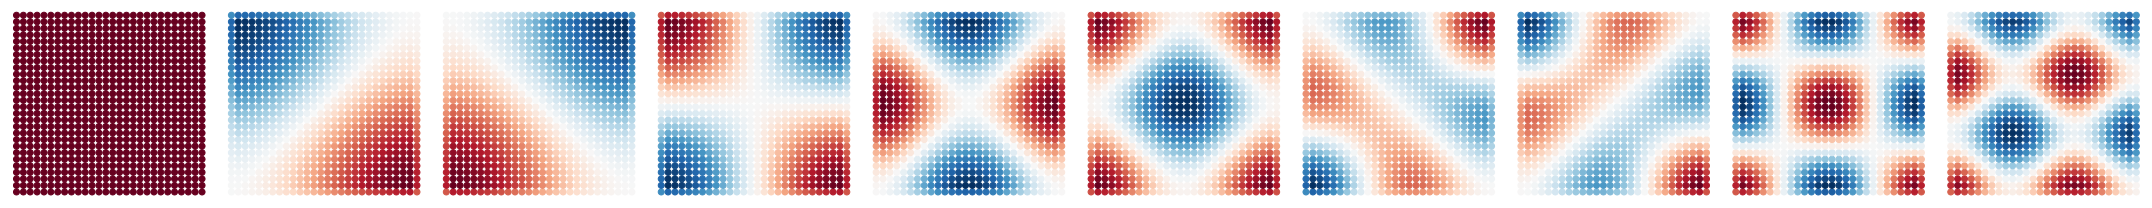
\includegraphics[width=\textwidth]{Images/r2_eigenvecs.png}
        \caption{Eigenvectors of the $[0,1]^2$ space, from $\phi_0$ (left) to $\phi_9$ (right).}
    \end{subfigure}
    \caption{Eigenmaps of the $[0,1]^2$ space.}
    \label{fig:r2_eigenmaps}
\end{figure*}



\begin{figure*}[h!] 
    \centering
    \begin{subfigure}[b]{0.9\textwidth}
        \centering
        \begin{tikzpicture}
        \begin{axis}[
            width=8cm, 
            height=4cm,
            xlabel={$k$},
            ylabel={$\lambda_k$},
            yticklabel style={
                    /pgf/number format/fixed,
                    /pgf/number format/precision=5
            },
            scaled y ticks=false
            ]
            \addplot[only marks, color=color2, mark size=1] table {Data/se2_eigenval.dat};
        \end{axis}
        \end{tikzpicture}
        \caption{Eigenvalues of the $[0,1]^2 \times [-\pi/2, \pi/2)$ space, from $\lambda_0$ to $\lambda_{49}$.}
    \end{subfigure}
    \hfill
    \begin{subfigure}[b]{\textwidth}
        \centering
        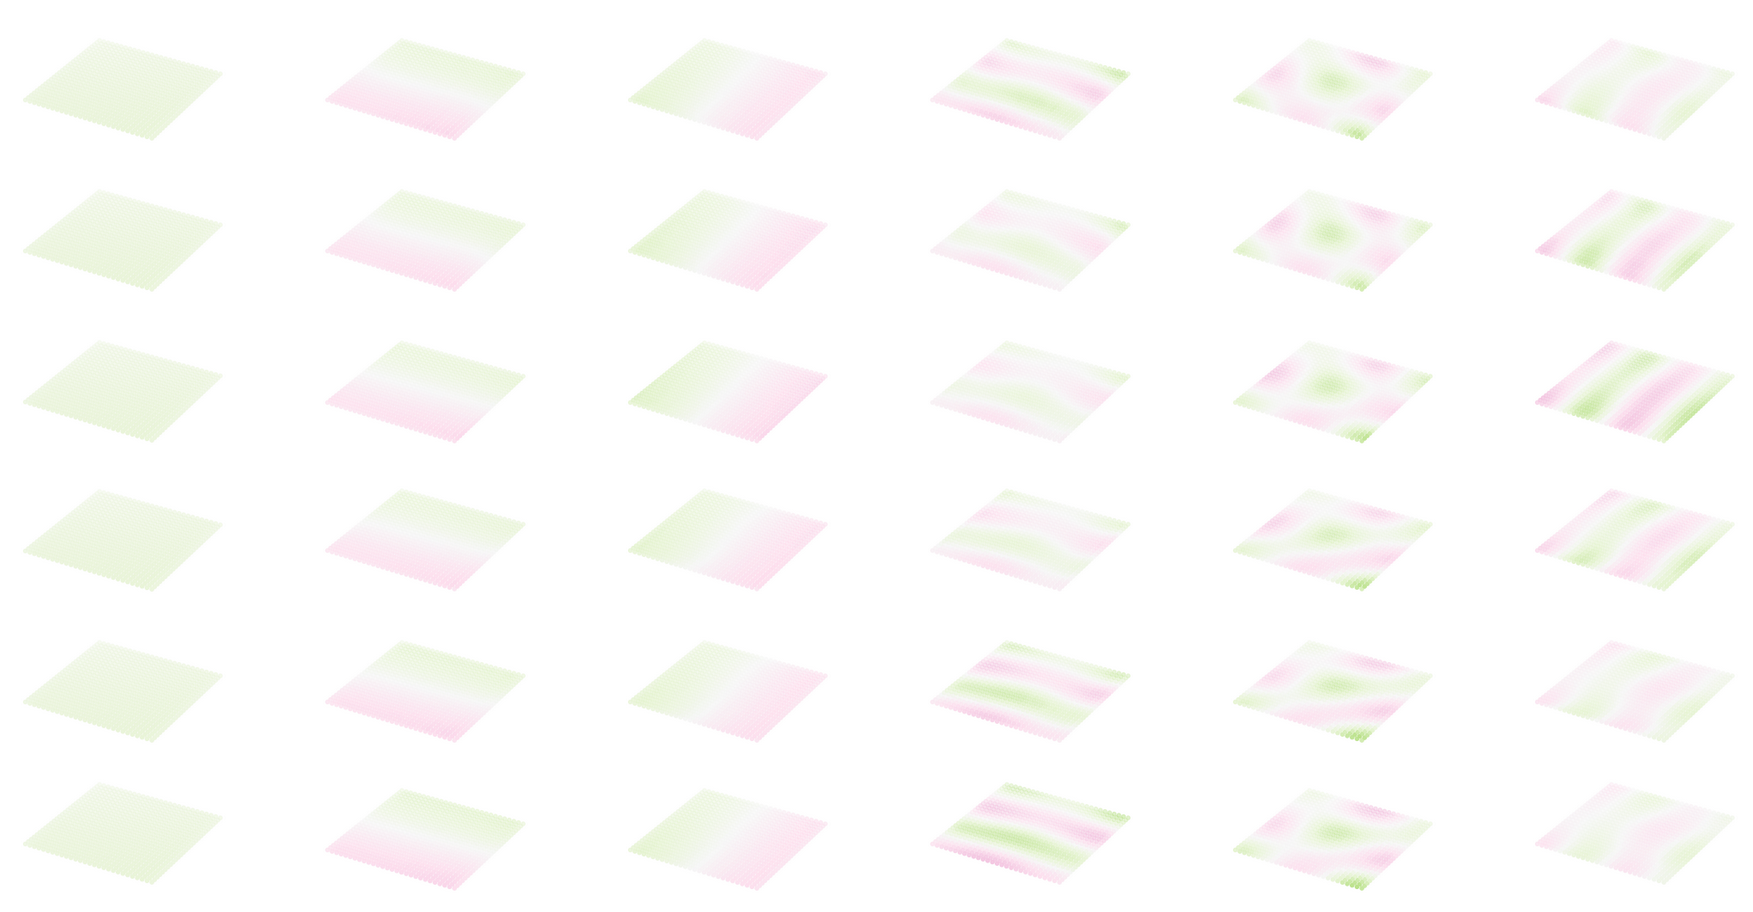
\includegraphics[width=\textwidth]{Images/se2_eigenvecs.png}
        \caption{Eigenvectors of the $[0,1]^2 \times [-\pi/2, \pi/2)$ space, from $\phi_0$ (left) to $\phi_9$ (right).}
    \end{subfigure}
    \caption{Eigenmaps of the $[0,1]^2 \times [-\pi/2, \pi/2)$ space.}
    \label{fig:se2_eigenmaps}
\end{figure*}


\begin{figure*}[h!] 
    \centering
    \begin{subfigure}[b]{0.9\textwidth}
        \centering
        \begin{tikzpicture}
        \begin{axis}[
            width=8cm, 
            height=4cm,
            xlabel={$k$},
            ylabel={$\lambda_k$},
            ]
            \addplot[only marks, color=color2, mark size=1] table {Data/s2_eigenval.dat};
        \end{axis}
        \end{tikzpicture}
        \caption{Eigenvalues of the $S^2$ space, from $\lambda_0$ to $\lambda_{49}$.}
    \end{subfigure}
    \hfill
    \begin{subfigure}[b]{\textwidth}
        \centering
        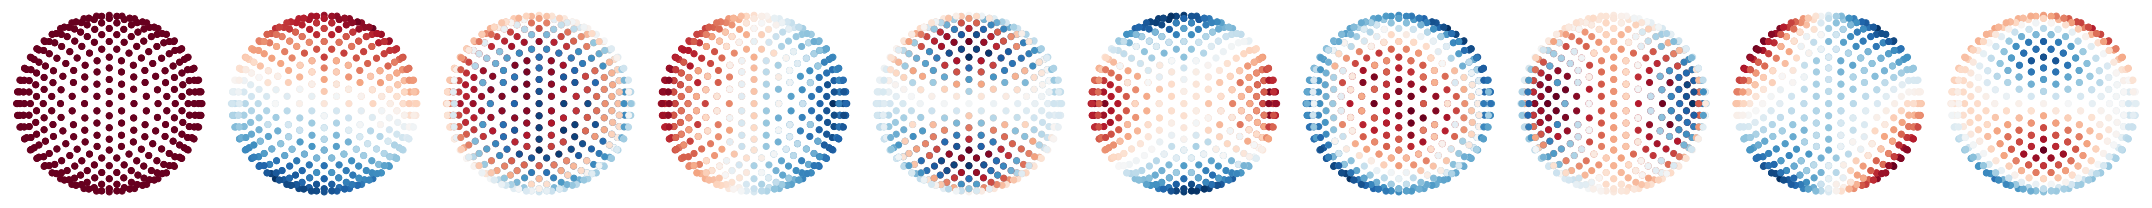
\includegraphics[width=\textwidth]{Images/s2_eigenvecs.png}
        \caption{Eigenvectors of the $S^2$ space, from $\phi_0$ (left) to $\phi_9$ (right).}
    \end{subfigure}
    \caption{Eigenmaps of the $S^2$ space.}
    \label{fig:s2_eigenmaps}
\end{figure*}

\begin{figure*}[h!] 
    \centering
    \begin{subfigure}[b]{0.9\textwidth}
        \centering
        \begin{tikzpicture}
        \begin{axis}[
            width=8cm, 
            height=4cm,
            xlabel={$k$},
            ylabel={$\lambda_k$},
            ]
            \addplot[only marks, color=color2, mark size=1] table {Data/so3_eigenval.dat};
        \end{axis}
        \end{tikzpicture}
        \caption{Eigenvalues of the $S^2 \times [-\pi/2, \pi/2)$ space, from $\lambda_0$ to $\lambda_{49}$.}
    \end{subfigure}
    \hfill
    \begin{subfigure}[b]{\textwidth}
        \centering
        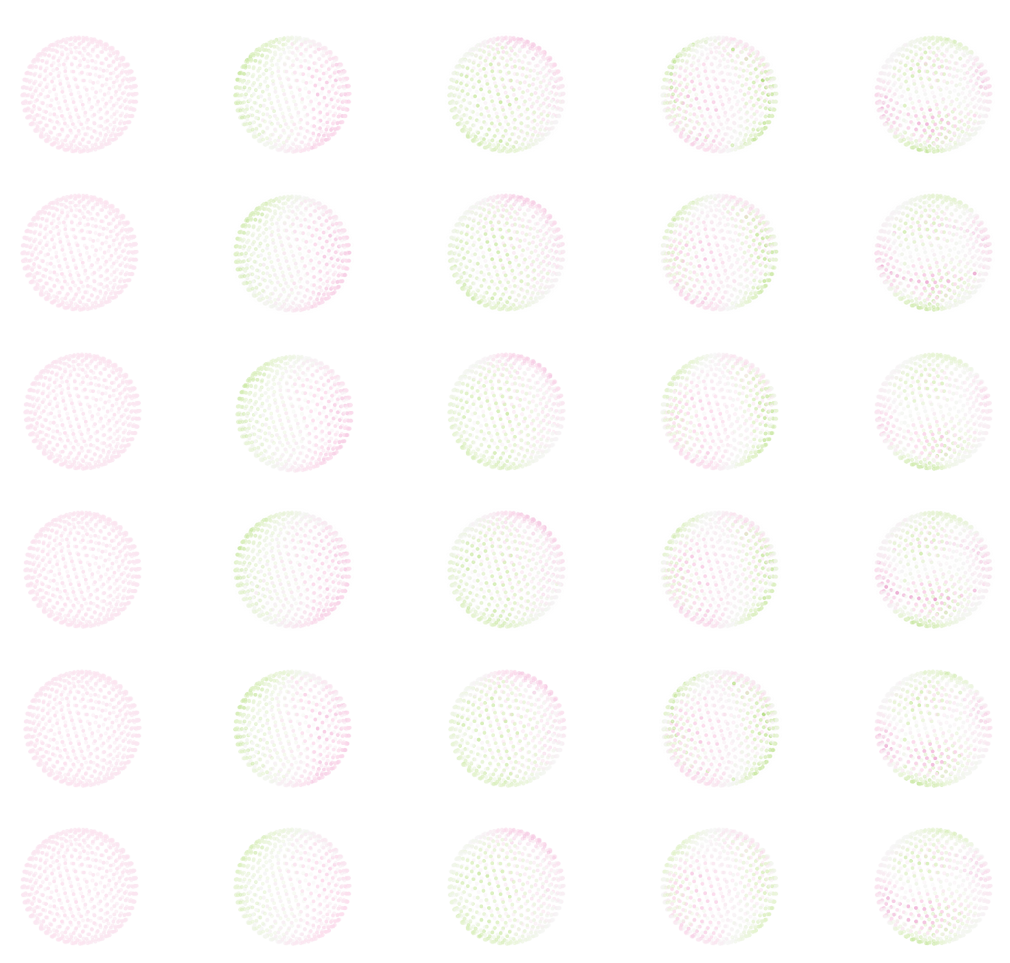
\includegraphics[width=\textwidth]{Images/so3_eigenvecs.png}
        \caption{Eigenvectors of the $S^2 \times [-\pi/2, \pi/2)$ space, from $\phi_0$ (left) to $\phi_9$ (right).}
    \end{subfigure}
    \caption{Eigenmaps of the $S^2 \times [-\pi/2, \pi/2)$ space.}
    \label{fig:so3_eigenmaps}
\end{figure*}




\clearpage

\section{Experiment details} \label{app:experiment_details}

Empirical evidence showed that deep and wide neural networks are keys to good performances. To help going deeper we used residual convolutional layers \citep{he2016deep} and batch normalization \citep{ioffe2015batch}. To avoid tuning of the learning rate, we use ADAM optimizers \citep{kingma2014adam} for all our experiments. Last, we initialise our models' parameters via the Kaiming method \citep{he2015delving}. 

\paragraph{Stability test on MNIST.} In these experiments, we used a Wide Residual ChebNet with three convolutional residual layers with rectified linear units and kernel of size $4$. As we do not pool at all, we only define one $SE(2)$ 16-NN graph with $28 \times 28 \times 6 = 4704$ vertices. We use extreme spatial anisotropy with $\varepsilon = 0.1$ and reach the 40/60 ratio using $\xi = 0.0026$. The residual layers are followed by a projective global max pooling layer and a fully connected with LogSoftMax output layer. 

\paragraph{Orientation anisotropic test on CIFAR10.} In these experiments, we used a Wide Residual ChebNet with three residual layers with rectified linear units and kernel of size $4$. We use two R2RandPool layers. Hence we define three $SE(2)$ 16-NN graphs with $32 \times 32 \times 6= 6144$, $16 \times 16 \times 6 = 1536$, and $8 \times 8 \times 6 = 384$ vertices. We use extreme spatial anisotropy with $\varepsilon = 0.1$. The residual layers are followed by a projective global max pooling layer and a fully connected with LogSoftMax output layer. 

\paragraph{Spatial anisotropic test on CIFAR10.} In these experiments, we used a Wide Residual ChebNet with 3 residual layers with rectified linear units and kernel of size $4$. We use two R2RandPool layers. Hence we define three $SE(2)$ 16-NN graphs with $32 \times 32 \times 6= 6144$, $16 \times 16 \times 6 = 1536$, and $8 \times 8 \times 6 = 384$ vertices. We use moderate orientation anisotropies to reach the 40/60 ratio on each graphs with $\xi \in \{0.002, 0.008, 0.016\}$. The isotropic case is constructed using $\varepsilon = \xi = 1$ on three $\mathbb{R}^2$ 8-NN graphs with $32 \times 32 \times 1 = 784$, $16 \times 16 \times 1 = 256$, and $8 \times 8 \times 1 = 64$ vertices. The residual layers are followed by a projective global max pooling layer and a fully connected with LogSoftMax output layer.

\paragraph{Scalability test on STL10.} In these experiments, we used a Wide Residual ChebNet with three residual layers with rectified linear units and kernel of size $4$. We use two R2RandPool layers. Hence we define three $SE(2)$ 16-NN graphs with $96 \times 96 \times 6= 55296$, $48 \times 48 \times 6 = 13824$, and $8 \times 8 \times 6 = 3456$ vertices. We use extreme spatial anisotropy with $\varepsilon = 0.1$ and reach the 40/60 ratio on each graphs using $\xi \in \{0.0002, 0.0009, 0.0036\}$. The isotropic case is constructed using $\varepsilon = \xi = 1$ on three $\mathbb{R}^2$ 8-NN graphs with $96 \times 96 \times 1 = 9216$, $48 \times 48 \times 1 = 2304$, and $24 \times 24 \times 1 = 576$ vertices. The residual layers are followed by a projective global max pooling layer and a fully connected with LogSoftMax output layer. The residual layers are followed by a projective global max pooling layer and a fully connected with LogSoftMax output layer. 

\paragraph{Scalability test on ClimateNet.} In these experiments, we used a U-ChebNet with three residual layers with rectified linear units and kernel of size $3$. We use five S2MaxPool (encoding) and five S2AvgUnpool (decoding) layers. Hence we define six $SO(3)$ 16-NN graphs with $10242 \times 6= 61452$, $2562 \times 6 = 15372$, $642 \times 6 = 3852$, $162 \times 6 = 972$, $42 \times 6 = 252$, and $12 \times 6 = 72$ vertices. We use extreme spatial anisotropy with $\varepsilon = 0.1$ and and reach the 40/60 ratio on each graphs using $\xi \in \{0.001, 0.004, 0.0156, 0.0617, 0.2381, 0.8333\}$. The residual layers are followed by a projective global max pooling layer and a fully connected with LogSoftMax output layer. 

\clearpage

\section{Stability under random perturbations}

In sensitive domains, the stability of a neural network to random perturbation is a desired property. We aim at demonstrate the high stability of our approach, as random perturbations are added to graphs during the training. We introduce two methods, both consisting in randomly pruning the original graph to construct a random sub-graph. At test time, random perturbations are removed in order to evaluate the model at its full capacity. 

\paragraph{Edges-based random subgraph.} 
A random sub-graph is created by randomly removing edges of the original graph. Based on the weights of the edges, a rate $1 - \kappa_\mathcal{E}$ of edges\footnote{Recently, \cite{keriven2020convergence} studied the convergence of quasi-sparse large random graphs to their continuous counterpart as the number of vertices grows. A direct consequence of their work is that even by randomly sampling the graph's edges, the graph Laplacian still remain consistent.} are discarded. It might be the case that a vertice becomes isolated during the process, meaning that all edges from and to this vertex have disappeared. It is not necessarily a problem, but it is important to be aware of this effect. 
\paragraph{Vertices-based random subgraph.}  
A random sub-graph is created by randomly removing a rate $1-\kappa_\mathcal{V}$ of vertices of the original graph. For the pruning being complete, edges from or to a discarded vertex should also be removed. This method is more drastic and should be used carefully, as such a vertices pruning leads to a violation of the uniform distribution of vertices that is required for consistency of the graph Laplacian. 

\begin{figure*}[h!] 
    \centering
    \begin{subfigure}[b]{0.48\textwidth}
        \centering
        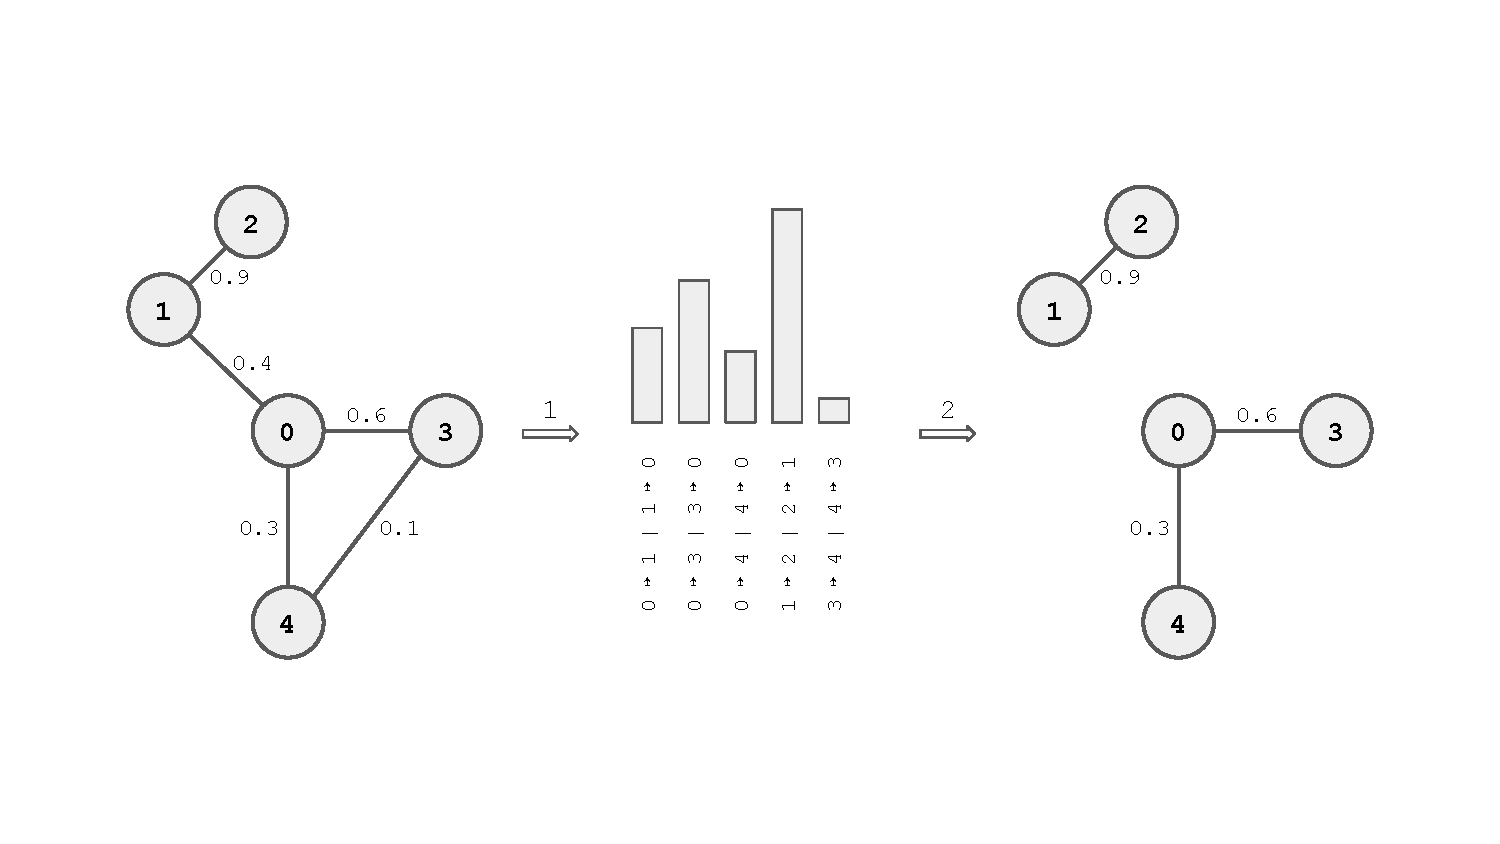
\includegraphics[width=\textwidth]{Images/edge_sampling.pdf}
        \caption{Edges sampling method with $\kappa_\mathcal{E} = 0.6$: 1) a p.m.f. based on the edges' weight is computed 2) $\kappa_\mathcal{E} |\mathcal{E}|$ are sampled according to the p.m.f.}
    \end{subfigure}
    \hfill
    \begin{subfigure}[b]{0.48\textwidth}
        \centering
        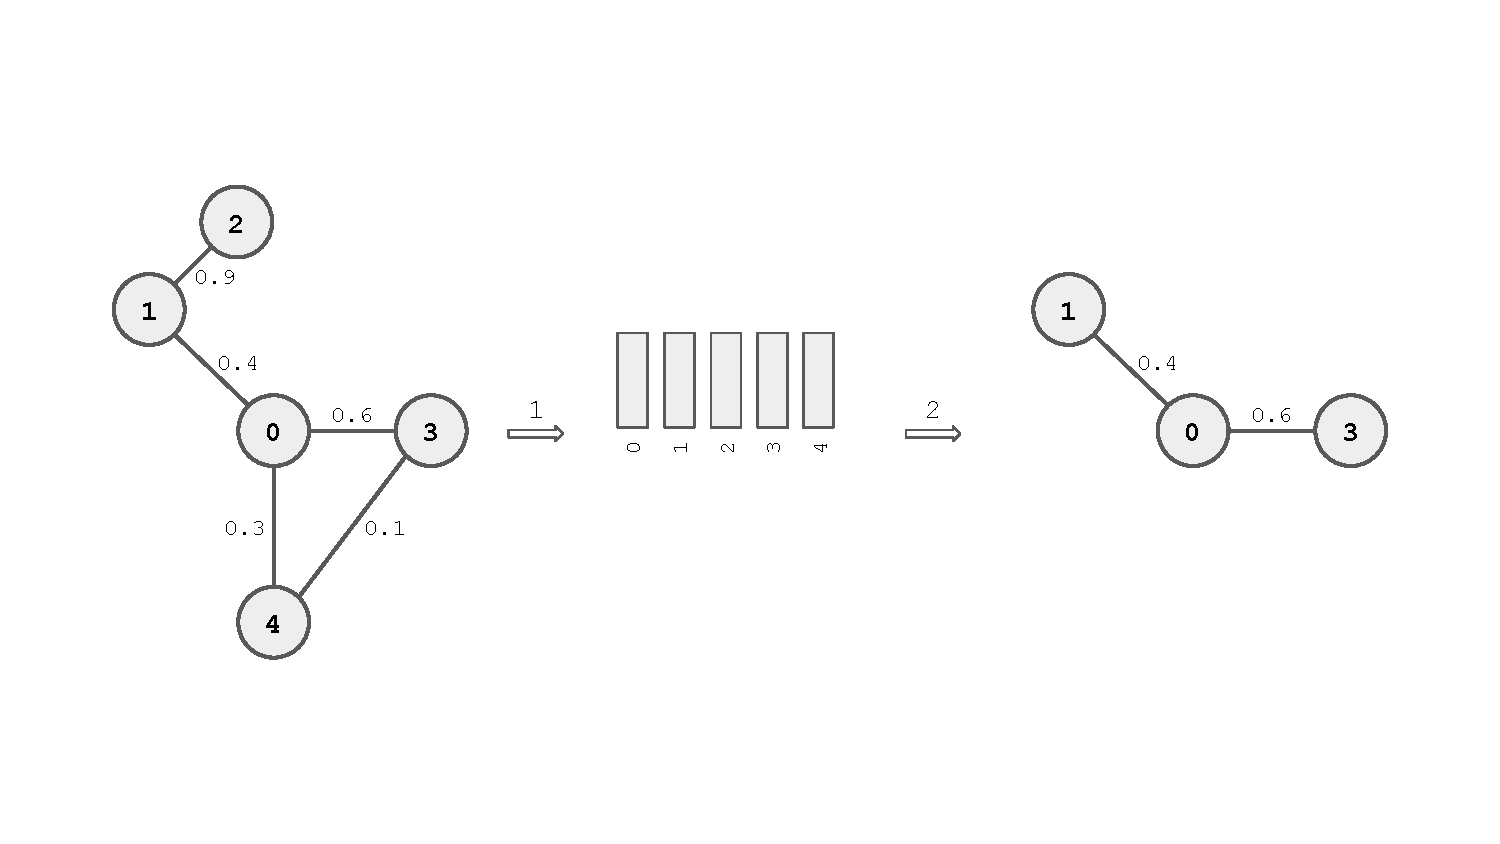
\includegraphics[width=\textwidth]{Images/vertex_sampling.pdf}
        \caption{Vertices sampling method with $\kappa_\mathcal{V} = 0.6$: 1) a uniform p.m.f. over the vertices is computed 2) $\kappa_\mathcal{V} |\mathcal{V}|$ are sampled according to the p.m.f.}
    \end{subfigure}
    \caption{Edges and vertices sampling methods.}
    \label{fig:sampling}
\end{figure*}

We run different experiments with a Wide Residual architecture on MNIST \citep{lecun1998gradient}, varying the rates of edges or vertices to sample. The objective of these experiments is twofold. First, we would like to test the stability of the model under random perturbations. Second, this experiment is also a good manner to demonstrate the equivariance property of our method. In this purpose, we train our model on the original training set of MNIST, adding some perturbations. At test time, we evaluate the model on the original test set with or without random rotations. 

\begin{figure*}[h!] 
    \centering
    \begin{subfigure}[b]{0.48\textwidth}
        \centering
        \caption{Test-accuracy against rate of edges to sample}
        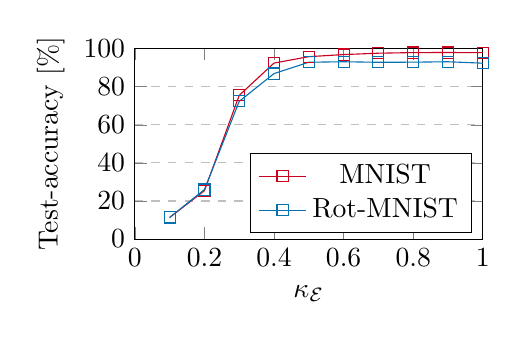
\begin{tikzpicture}
        \begin{axis}[
            xlabel={$\kappa_{\mathcal{E}}$},
            ylabel={Test-accuracy [\%]},
            xmin=0, xmax=1,
            ymin=0, ymax=100,
            xtick={0,0.2,0.4,0.6,0.8,1.0},
            ytick={0,20,40,60,80,100},
            legend pos=south east,
            ymajorgrids=true,
            grid style=dashed,
            width=6cm,
            height=4cm
        ]
        
        \addplot[
            color=color1,
            mark=square,
            ]
            coordinates {
            (0.1,11.35)(0.2,25.42)(0.3,75.49)(0.4, 92.43)(0.5,95.79)(0.6,96.89)(0.7,97.61)(0.8,97.94)(0.9,97.96)(1.0,97.92)
            };
            \addlegendentry{MNIST}
            
        \addplot[
            color=color2,
            mark=square,
            ]
            coordinates {
            (0.1,11.35)(0.2,26.00)(0.3,72.33)(0.4, 86.91)(0.5,92.87)(0.6,93.12)(0.7,92.84)(0.8,92.90)(0.9,93.12)(1.0,92.37)
            };
            \addlegendentry{Rot-MNIST}
        \end{axis}
        \end{tikzpicture}
    \end{subfigure}
    \hfill
    \begin{subfigure}[b]{0.48\textwidth}
        \centering
        \caption{Test-accuracy against rate of vertices to sample}
        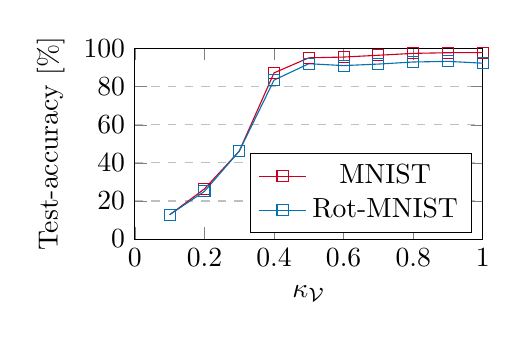
\begin{tikzpicture}
        \begin{axis}[
            xlabel={$\kappa_{\mathcal{V}}$},
            ylabel={Test-accuracy [\%]},
            xmin=0, xmax=1,
            ymin=0, ymax=100,
            xtick={0,0.2,0.4,0.6,0.8,1.0},
            ytick={0,20,40,60,80,100},
            legend pos=south east,
            ymajorgrids=true,
            grid style=dashed,
            width=6cm,
            height=4cm
        ]
        
        \addplot[
            color=color1,
            mark=square,
            ]
            coordinates {
            (0.1,12.75)(0.2,26.34)(0.3,46.15)(0.4, 87.27)(0.5,95.18)(0.6,95.59)(0.7,96.53)(0.8,97.52)(0.9,97.87)(1.0,97.92)
            };
            \addlegendentry{MNIST}
            
        \addplot[
            color=color2,
            mark=square,
            ]
            coordinates {
            (0.1,12.81)(0.2,25.04)(0.3,46.15)(0.4, 83.48)(0.5,92.09)(0.6,91.1)(0.7,91.9)(0.8,92.99)(0.9,93.32)(1.0,92.37)
            };
            \addlegendentry{Rot-MNIST}
        \end{axis}
        \end{tikzpicture}
    \end{subfigure}
    \caption{Stability and group equivariance under random perturbations.}
\end{figure*}

\haguettaz{
Comments and discussion:
\begin{itemize}
\item We observe empirical almost-equivariance\footnote{Basically, the equivariance error of an operator could be decomposed in two terms: an extrinsic and an intrinsic errors. The intrisic error is the error we are trying to measure, it is the equivariance error due to the operators itself. The extrinsic error is the error caused by the testing method itself, in the semantic of the data (e.g. is it always possible to differentiate a six from a nine without orientation information?) or numerical artificats (e.g. how to rotate a low resolution image by 10 degrees without alteration?). In general, we only have access to the total equivariance error.} of the model over rotations. With a similar experiment with random flips, we could also check that the model is equivariant under flips.
\item Random perturbations does not help in reaching higher performances in this case. Nevertheless, our hypothesis is that is that it could help struggling overfitting as it is a dropout-like method. It does not seems to change the training duration as the consumed time when perturbing the graph is make up during the forward and backward passes as the graph Laplacian became sparser.
\item The rate of edges or vertices to sample greatly impact the performance of the model. However, we notice that the model remains stable even at middle-low rates of sampling. At low rates, the information flows throughout the graphs are too disturbed to let the model learn anything. We should also be aware that the effect of the sampling rates also depends on the connectivity of the graph. Indeed, as the number of edges increases, we should theoretically use an lower sampling rate as the flow throughout a highly connected graph is less impacted by random closures of edges or vertices. We conclude that more edges capture the geometry better but with diminishing returns. Therefore, there is not point to use a fully connected graph.
\end{itemize}
}
\end{document}
